\chapter{RESULTS}

\section{RESULTS}
In order to give a detailed display of the flexibility of this method, we wanted to show the results of the method after changing many of the parameters.  These include varying the resolution of the screen, angle of between VPL rays, number of VPL's per ray, and number of indirect shadow maps used. Modifying these parameters will have an impact on performance or number of frames rendered per second as well as quality.  Therefore, section \ref{sec:fps} will detail the performance impact of varying the parameters based off the change in the number of frames per second rendered and section \ref{sec:quality} will detail the impact of varying the parameters on the quality of the images rendered by calculating the percentage difference per pixel against the default parameter set-up.  As a reminder, the default method which is featured first on each table uses a resolution size of 1280 by 720, an angle of 5 degrees between VPL rays, 5 VPL's per ray, and 20 indirect shadow maps.

\subsection{IMPACT OF PARAMETER CHOICES ON FPS} \label{sec:fps}
The results will given in frames per second (FPS).  Table \ref{table:5.1} will display the results of varying the angle between the VPL rays. Table \ref{table:5.2} will display the results of varying the number of VPL's used on each ray (the total number of hemispheres). Table \ref{table:5.3} will display the results of using varying the resolution used.  Lastly, \ref{table:5.4} will display the results of reducing the number of indirect shadow maps used.

\begin{table}[h!]
	\caption{Varying the Angle Between VPL Rays (Impact on FPS)}
	\begin{center}
	    \begin{tabular}{ | l | l | l | l | l | l |}
	    \hline
	    Resolution & Angle & VPL's Per Ray & Total \#VPL's & \#Indirect SM's & FPS\\ \hline
	    1280x720 & 5 & 5 & 6485 & 20 & 55\\ \hline
	    1280x720 & 10 & 5 & 1625 & 20 & 65\\ \hline
	    1280x720 & 30 & 5 & 185 & 20 & 84\\ \hline
	    1280x720 & 45 & 5 & 85 & 20 & 95\\ \hline
	    1280x720 & 90 & 5 & 25 & 20 & 100\\ \hline
	    \end{tabular}
	\end{center}
	\label{table:5.1}
\end{table}

\begin{table}[h!]
	\caption{Varying the Number of VPL's Per Ray (Impact on FPS)}
	\begin{center}
	    \begin{tabular}{ | l | l | l | l | l | l |}
	    \hline
	    Resolution & Angle & VPL's Per Ray & Total \#VPL's & \#Indirect SM's & FPS\\ \hline
	    1280x720 & 5 & 5 & 6485 & 20 & 55\\ \hline
	    1280x720 & 5 & 4 & 5188 & 20 & 56\\ \hline
	    1280x720 & 5 & 3 & 3891 & 20 & 61\\ \hline
	    1280x720 & 5 & 2 & 2594 & 20 & 62\\ \hline
	    1280x720 & 5 & 1 & 1297 & 20 & 78\\ \hline
	    1280x720 & 5 & 6 & 7782 & 20 & 52\\ \hline
	    \end{tabular}
	\end{center}
	\label{table:5.2}
\end{table}

\begin{table}[h!]
	\caption{Varying the Resolution Size. (Impact on FPS)}
	\begin{center}
	    \begin{tabular}{ | l | l | l | l | l | l |}
	    \hline
	    Resolution & Angle & VPL's Per Ray & Total \#VPL's & \#Indirect SM's & FPS\\ \hline
	    1280x720 & 5 & 5 & 6485 & 20 & 55\\ \hline
	    1120x630 & 5 & 5 & 6485 & 20 & 82\\ \hline
	    960x540 & 5 & 5 & 6485 & 20 & 104\\ \hline
	    800x450 & 5 & 5 & 6485 & 20 & 119\\ \hline
	    640x360 & 5 & 5 & 6485 & 20 & 133\\ \hline
	    1440x810 & 5 & 5 & 6485 & 20 & 42\\ \hline
	    \end{tabular}
	\end{center}
	\label{table:5.3}
\end{table}

\begin{table}[h!]
	\caption{Varying the Number of Indirect Shadow Maps (Impact on FPS)}
	\begin{center}
	    \begin{tabular}{ | l | l | l | l | l | l |}
	    \hline
	    Resolution & Angle & VPL's Per Ray & Total \#VPL's & \#Indirect SM's & FPS\\ \hline
	    1280x720 & 5 & 5 & 6485 & 20 & 55\\ \hline
	    1280x720 & 5 & 5 & 6485 & 15 & 87\\ \hline
	    1280x720 & 5 & 5 & 6485 & 10 & 106\\ \hline
	    1280x720 & 5 & 5 & 6485 & 5 & 128\\ \hline
	    1280x720 & 5 & 5 & 6485 & 1 & 157\\ \hline
	    1280x720 & 5 & 5 & 6485 & 0 & 161\\ \hline
	    \end{tabular}
	\end{center}
	\label{table:5.4}
\end{table}

Tables \ref{table:5.1}, \ref{table:5.2}, \ref{table:5.3}, and \ref{table:5.4} show some important characteristics.  First, tables \ref{table:5.1} and \ref{table:5.2} shows the impact of the angle between rays and the number of VPL's per ray on the total number of VPL's used.  The equation to calculate the total number of VPL's based off the angle and the number of VPL's per ray used is:

\begin{equation}
numberVPLs = VPLsPerRay*((90/Angle)*(360/Angle)+1)
\label{eqn:calcVPLtotal}
\end{equation}

More interestingly, it shows that a large difference between the total number of VPL's used has a relatively small affect on the FPS recorded compared to other changes.  For example, reducing the number of VPL's used by a factor of 4 (from 6485 to 1625) increases FPS by only 10 whereas reducing the number of VPL's used by a factor of near 76 (from 6485 to 85) increases FPS by 40.

Table \ref{table:5.3} shows that decreasing the resolution of the screen has a relatively large impact on the FPS recorded.  To compare it against decreasing the number of VPL's used, in order to see a similar impact of reducing the resolution by 77\% or a factor of 1.3, we would have to reduce the number of VPL's by a factor of 35 (from 6485 to 185).

Similarly, table \ref{table:5.4} shows the number of indirect shadow maps having a relatively large impact on the performance.  As mentioned often in similar studies on indirect illumination, calculating indirect shadows is computationally expensive as supported in table \ref{table:5.4}.  To make a similar comparison as above, reducing the number of shadow maps used by 5, a factor of 1.33 or 75\%, has a similar impact as reducing the resolution by 77\% or a factor of 1.3 or reducing the number of VPL's by a factor of 35 (from 6485 to 185).  Also, table \ref{table:5.4} shows that for each indirect shadow map we add, we can expect a decrease in FPS by about 5.

In summary, when choosing parameters of the method to be run on slower machines, a combination of reducing the resolution and reducing the number of indirect shadow maps would result in the most efficient performance gain in regards to FPS increase.  Next, we will similarly analyze the impact of these parameter changes to the quality of the image in order to see what changes would result in the most efficient reductions while maintaining quality.

\subsection{IMPACT OF PARAMETER CHOICES ON QUALITY} \label{sec:quality}
Just as important as performance is the quality of the images rendered.  Therefore, this section will detail the quality impact of parameter choice using the default set-up as the reference image.  By detailing this information, it will reveal the ultimate flexibility of the method and whether we can use this method on slower machines with limited quality impact.  We will use the same parameter choices as the tables for section \ref{sec:fps}, but we will be interested in the percentage difference between the chosen parameters and the default parameters.  The percentage difference will be computed using a Python script which takes in two rendered images as input and compares them on a pixel by pixel basis.  This comparison is done as follows:


\begin{algorithm}[H]
 \SetAlgoLined
 similar = 0.0\;
 \For{each pixelComponent (R,B,G) in image 1}{
  \eIf{pixelComponent\_image1 $>=$ pixelComponent\_image2 }{
   similar += (pixelComponent\_image1 +1) / (pixelComponent\_image2 +1)\;
   }{
   similar += (pixelComponent\_image2 +1) / (pixelComponent\_image1 +1)\;
  }
 }
 similar = similar/numPixelComponents\;
 percentDifference = (1-similar)*100\;
 \caption{Compute Image Difference}
 \label{alg:difference}
\end{algorithm}

Algorithm \ref{alg:difference} adds 1 to the 2 pixel components in order to avoid division by 0.  This way our pixel components will range from 1 to 256.  For example, if image 1 had a value of 200 for the red component of pixel 1 and image 2 had a value of 100 for the red component of pixel 1, we would say that these two images were 50\% different.  We do this calculation for all 3 color components of every pixel in each image and average it out to find the total similarity or difference between the two images.

The purpose of doing such a calculation is simply due to the fact that quantifying the quality of an image or  the similarity with another image is rather subjective.  This way we can assign a value to the comparison which is more objective.  This way we can objectively order the images rendered using different parameters by similarity to the default parameter set-up and declare certain parameter changes as more efficient than others.  By efficient, we mean the parameter changes increase performance with limited quality reductions.  Tables \ref{table:5.5}, \ref{table:5.6}, \ref{table:5.7}, and \ref{table:5.8} show the calculated similarity percentages.  The higher percentage the image, the closer to the reference image it is with 100\% meaning that it is the same image.


\begin{table}[h!]
	\caption{Varying the Angle Between VPL Rays (Impact on Quality)}
	\begin{center}
	    \begin{tabular}{ | l | l | l | l | l | l |}
	    \hline
	    Resolution & Angle & VPL's Per Ray & Total \#VPL's & \#Indirect SM's & \% Similar\\ \hline
	    1280x720 & 5 & 5 & 6485 & 20 & 100\\ \hline
	    1280x720 & 10 & 5 & 1625 & 20 & 97.945\\ \hline
	    1280x720 & 30 & 5 & 185 & 20 & 97.956\\ \hline
	    1280x720 & 45 & 5 & 85 & 20 & 95.440\\ \hline
	    1280x720 & 90 & 5 & 25 & 20 & 92.676\\ \hline
	    \end{tabular}
	\end{center}
	\label{table:5.5}
\end{table}

\begin{table}[h!]
	\caption{Varying the Number of VPL's Per Ray (Impact on Quality)}
	\begin{center}
	    \begin{tabular}{ | l | l | l | l | l | l |}
	    \hline
	    Resolution & Angle & VPL's Per Ray & Total \#VPL's & \#Indirect SM's & \% Similar\\ \hline
	    1280x720 & 5 & 5 & 6485 & 20 & 100\\ \hline
	    1280x720 & 5 & 4 & 5188 & 20 & 92.973\\ \hline
	    1280x720 & 5 & 3 & 3891 & 20 & 93.458\\ \hline
	    1280x720 & 5 & 2 & 2594 & 20 & 90.318\\ \hline
	    1280x720 & 5 & 1 & 1297 & 20 & 91.591\\ \hline
	    1280x720 & 5 & 6 & 7782 & 20 & 96.509\\ \hline
	    \end{tabular}
	\end{center}
	\label{table:5.6}
\end{table}

\begin{table}[h!]
	\caption{Varying the Resolution Size. (Impact on Quality)}
	\begin{center}
	    \begin{tabular}{ | l | l | l | l | l | l |}
	    \hline
	    Resolution & Angle & VPL's Per Ray & Total \#VPL's & \#Indirect SM's & \% Similar\\ \hline
	    1280x720 & 5 & 5 & 6485 & 20 & 100\\ \hline
	    1120x630 & 5 & 5 & 6485 & 20 & 99.547\\ \hline
	    960x540 & 5 & 5 & 6485 & 20 & 99.541\\ \hline
	    800x450 & 5 & 5 & 6485 & 20 & 99.418\\ \hline
	    640x360 & 5 & 5 & 6485 & 20 & 99.483\\ \hline
	    1440x810 & 5 & 5 & 6485 & 20 & 99.741\\ \hline
	    \end{tabular}
	\end{center}
	\label{table:5.7}
\end{table}

\begin{table}[h!]
	\caption{Varying the Number of Indirect Shadow Maps (Impact on Quality)}
	\begin{center}
	    \begin{tabular}{ | l | l | l | l | l | l |}
	    \hline
	    Resolution & Angle & VPL's Per Ray & Total \#VPL's & \#Indirect SM's & \% Similar\\ \hline
	    1280x720 & 5 & 5 & 6485 & 20 & 100\\ \hline
	    1280x720 & 5 & 5 & 6485 & 15 & 99.475\\ \hline
	    1280x720 & 5 & 5 & 6485 & 10 & 98.853\\ \hline
	    1280x720 & 5 & 5 & 6485 & 5 & 93.611\\ \hline
	    1280x720 & 5 & 5 & 6485 & 1 & 90.897\\ \hline
	    1280x720 & 5 & 5 & 6485 & 0 & 98.563\\ \hline
	    \end{tabular}
	\end{center}
	\label{table:5.8}
\end{table}

Comparing tables \ref{table:5.5} and \ref{table:5.6} reveals that although the number of VPL's used when increasing our VPL ray angles drops more quickly than when we simply reduce the number of VPL per ray, the higher ray angle images (table \ref{table:5.5}) render more similar images to the reference than when we reduce the number of VPL per ray.  For example, when we use 185 VPL's with an angle of 30 degrees, we get an image that is 98\% similar to the reference, but when we use 1297 VPL's with 1 VPL per ray, we get an image that is only 91.6\% similar to the reference.  This leads us to believe that increasing the angle to reduce the number of VPL's leads to better quality images than reducing the number of VPL's per ray or hemispheres to reduce the number of VPL's.  Such an observation can helps us increase performance and maintain a level of similarity to the reference image.

When looking at table \ref{table:5.7}, we see high values of similarity to the reference, however, these can be misleading.  These values were calculated after rendering the image at the chosen resolution size and then stretching it to the reference image resolution size.  This brings into question the idea of global similarity and local similarity as well as notion of visually pleasing as discussed in section \ref{sec:study}.  Although these images are very similar to the reference in an overall pixel by pixel basis, there are some things that this number does not show us.  It requires looking at the stretched image to realize the effect this has on the image quality.  These images show worsening cases of 'jaggies' or artifacts near the edges of boundaries such as the edges of the boxes as the rendered image's resolution gets smaller.  So in the regard of being similar to the reference these reduced resolution images are, but when stretched they also show localized differences that can be distracting to the eye.  When comparing the reference to the stretched 640x360 images on a local scale such as on the edges of a box, we get a similarity of 97.4\% which is slightly less than the 99.5\%, however, a even more localized comparison such as a few pixels on either side of the boundary line would show even more difference.

Regardless of the calculations, a localized difference such as artifacts detract from the overall realism of the image which is not preferred.  A slight global difference, however, such as a slightly lighter or darker overall image would result in a large difference value but more similar overall to the human eye.  These facts need to be taken into consideration when choosing the method or parameters.  This idea will be covered more in section \ref{sec:alternatives}.

Table \ref{table:5.8} shows the impact of reducing the number of shadow maps used for indirect shadows.  An interesting note is that when using 10 shadow maps for indirect shadows and when completely ignoring indirect shadows we get near identical similarity measurements to our reference.  This reinforces the notion that indirect shadows are possibly an unnecessary computational burden that can be ignored especially on slower machines.  Recall table \ref{table:5.4} and the comparison of FPS between the two parameter choices.  When choosing to use 10 indirect shadow maps we get 106 FPS, however, when we ignore indirect shadows we get 161 FPS.  For nearly identical globally similarity values, we can gain 55 FPS by ignoring indirect shadows.  This is a major parameter choice to consider when wanting to increase performance.

It is worth noting that if an image is not 100\%, this does not mean that it is not a quality or accurate image rendering.  It purely means that the image is in some way different to our reference image.  For example, the last entry of table \ref{table:5.6} says that it is 96.5\% similar to our reference.  However, due to the fact that this rendering indeed uses more VPL's than our reference, this image could be perceived as more accurate or of higher quality than our reference.  This calculation does take into account the findings of section \ref{sec:study} which stated that there was found to be a connection between the amount of indirect illumination and the perceived similarity to the reference.  More on the idea of the amount of indirect illumination will be discussed in section \ref{sec:alternatives}.

\subsection{ALTERNATIVES} \label{sec:alternatives}
The aim of this section is to determine any additional sacrifices that could be made in order to improve performance.  As shown in table \ref{table:5.8} and discussed above, indirect shadowing is the most computationally expensive scene component that has the least influence of the overall scene.  This may lead one to consider whether or not ignoring indirect lighting could be possible.  However, as shown in table \ref{table:5.9}, we compared our default method with a direct lighting only method.  Using our similarity calculation, we see the lowest similarity of 84.4\%, but the highest performance with 681 FPS.  On a machine that is able to run any of the above parameter choices with at least 30 FPS, it is not necessary to sacrifice this much quality for performance, but for the slowest machines, this may be a necessary choice.

\begin{table}[h!]
	\caption{Alternative Reductions}
	\begin{center}
	    \begin{tabular}{ | l | l | l | l | l | l |}
	    \hline
	    Method & FPS & \% Similarilty to Default\\ \hline
	    Default Method & 55 & 100\\ \hline
	    Direct Lighting ONLY & 681 & 84.426\\ \hline
	    Indirect Lighting w/out indirect shadows & 161 & 98.563\\ \hline
	    Faked Indirect Lighting (1.1x) & 681 & 88.217\\ \hline
	    Faked Indirect Lighting (1.2x) & 681 & 90.675\\ \hline
	    Faked Indirect Lighting (1.3x) & 681 & 91.847\\ \hline
	    Faked Indirect Lighting (1.4x) & 681 & 91.393\\ \hline
	    Faked Indirect Lighting (1.5x) & 681 & 90.161\\ \hline
	    \end{tabular}
	\end{center}
	\label{table:5.9}
\end{table}

Also in table \ref{table:5.9}, we include our indirect lighting without indirect shadows method for comparison with it's respectable 161 FPS and 98.5\% similarity.  This was the best performing parameter choice from tables \ref{table:5.1} through \ref{table:5.4}.  Should a compromise between direct lighting only and indirect lighting with no indirect shadows be needed, we included a few alternative approaches in addition to the previous two in table \ref{table:5.9}.  These approaches attempt to fake indirect lighting while achieving the direct only performance.  This is done through the use of scaling the color and shadow contributions in the fragment shader.  As reminded above and discovered in section \ref{sec:study}, the amount of indirect light can contribute to the perceived realism of the scene.  As such, 5 different scaling approaches are included in table \ref{table:5.9} to compare against our reference image.  The multiplier in parenthesis in each table entry shows the amount of scaling done to the direct lighting of the scene.  For example, for the entry with a 1.1 multiplier this means that the final color is calculated as below:

\begin{equation}
color = (direct\_color*0.5*shadow)+(direct\_color*0.6)
\end{equation}

For the next entry the 0.6 would be 0.7 and so on.  This way the direct shadows are only half as dark as before and is not purely black and increase the overall brightness of the scene.  As seen in the table, this approach of faking indirect light leads to better similarity numbers than using just the direct lighting approach peaking at the multiplier of 1.3 with a value of 91.8\% in this particular case.  Therefore, should indirect lighting without indirect shadows approach be too much for a particular machine, a faked version of indirect lighting would be a respectable compromise.

\subsection{FINAL ANALYSIS} \label{sec:finalAnalysis}
Lastly, we will consolidate all of the previous data and tables in order to determine the most efficient reductions and the most influencing factors on the believability of the rendered scene.  The benefits of calculating similarities is that it leads to a way of quantifying quality in comparison to our reference image and thus rank parameter choices based off a combination of performance gains and limited quality impact.  It is important to note that changing the resolution size and stretching netted the best similarity results, but due to the introduction of artifacts, those parameter choices will not be included.  It is also important to note that should a smaller resolution size be applicable without the need to stretch to our larger default resolution, this should be the very first choice in increasing performance, because the artifacts are only introduced during the stretching process due to the method of likely naive sampling.

Table \ref{table:5.10} will use the similarity values calculated along with the FPS gain in order to rank the parameter choices.  This will be done using a simple equation:

\begin{equation}
rankValue = fpsGain / (1-calculatedSimilarity)
\end{equation}

\begin{table}[h!]
	\caption{Final Comparisons}
	\begin{center}
	    \begin{tabular}{ | l | l | l | l | l | l |}
	    \hline
	    Method & FPS & \% Similarilty & Rank Value & Figure\\ \hline
	    Default Method & 55 & 100 & -- & \ref{fig:defaultimage}\\ \hline
	    Faked Indirect Lighting (1.3x) & 681 & 91.847 & 76.7816 & \ref{fig:fakedindirect}\\ \hline
	    Indirect Lighting w/out indirect shadows & 161 & 98.563 & 73.7648 & \ref{fig:0indSM}\\ \hline
	    Indirect Lighting w/ 15 indirect shadows & 87 & 99.475 & 60.9524 & \ref{fig:15indSM}\\ \hline
	    Indirect Lighting w/ 10 indirect shadows & 106 & 98.853 & 44.4638 & \ref{fig:10indSM}\\ \hline
	    Direct Lighting ONLY & 681 & 84.426 & 40.1952 & \ref{fig:directonly}\\ \hline
	    \hline
	    \hline
	    30 Degree Angle Between VPL Rays & 84 & 97.956 & 14.1879 & \ref{fig:VPLangleIncrease}\\ \hline
	    \hline
	    \hline
	    Reduction down to 1 VPL Per Ray & 78 & 91.591 & 2.7352 & \ref{fig:hemisphereReduction}\\ \hline
	    \hline
	    \hline
	    Resolution Reduction 640x360 & 133 & 99.483 & 150.8704 & \ref{fig:smallerresolution}\\ \hline
	    \end{tabular}
	\end{center}
	\label{table:5.10}
\end{table}

Table \ref{table:5.10} tells us a few things:
\begin{itemize}
\item If a smaller resolution size can be used and not stretched, use it.
\item Indirect Shadows are nice, but is the next thing to be sacrificed if better performance is needed.
\item If we chose to reduce VPL's, do so by increasing the ray angles, not by reducing hemispheres.
\item We can experiment with multipliers and get decent faked indirect lighting if nothing else.
\end{itemize}

\section{IMAGES}
This section will be used to show images captured from the real-time rendering produced using this method and the accompanying parameters chosen.


\begin{figure}[h!]
  \centering
    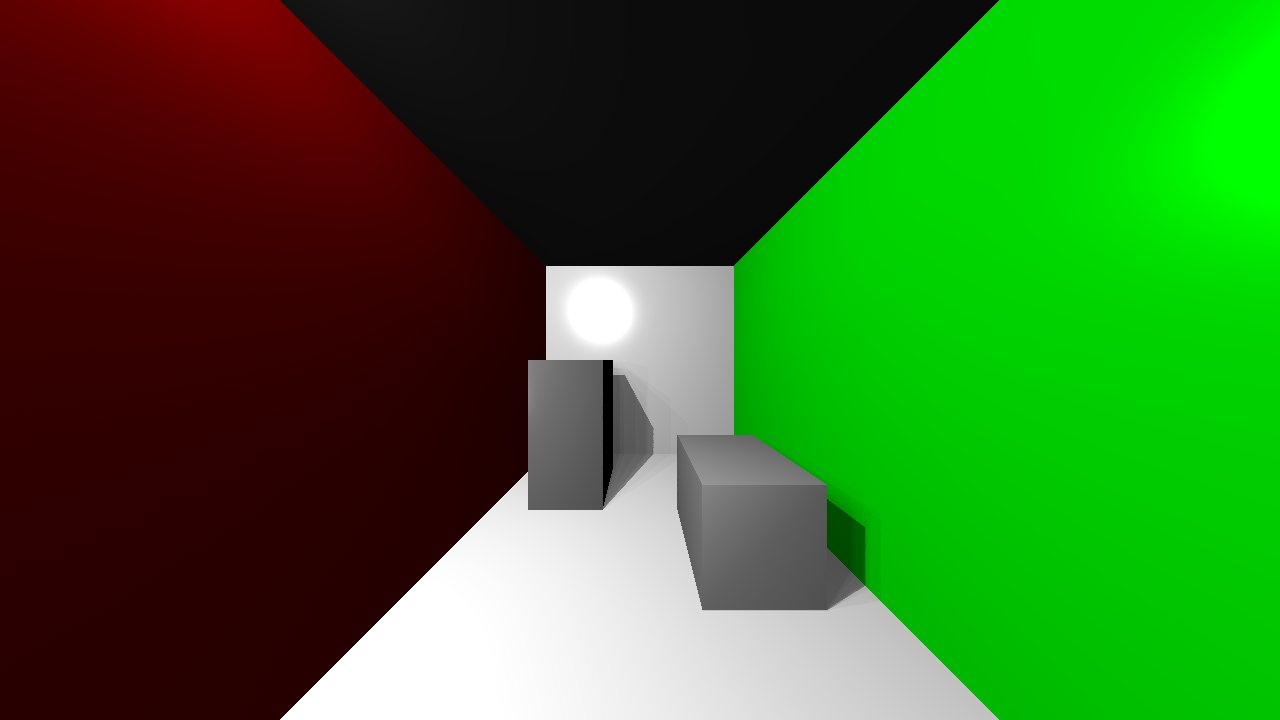
\includegraphics[width=1.0\textwidth]{sample1.jpg}
%    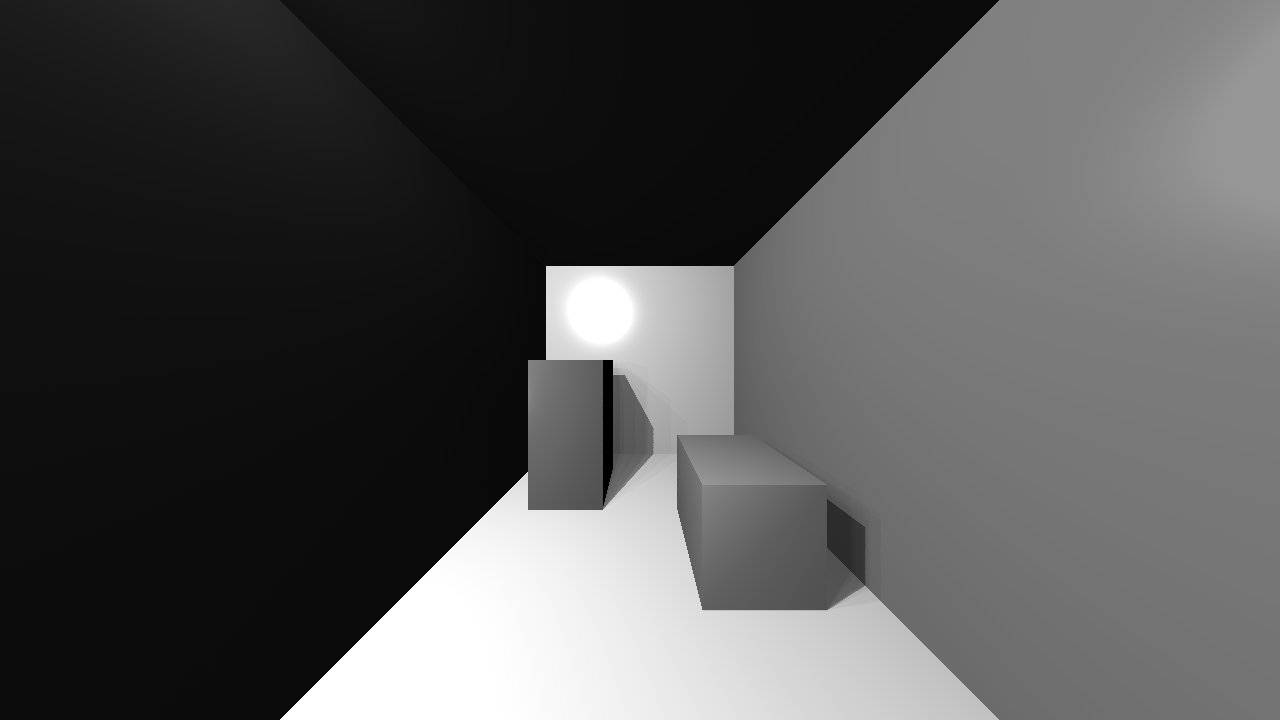
\includegraphics[width=1.0\textwidth]{sample1_gray.jpg}
  \caption{Light is at the near upper left corner of the scene. This image uses the default parameters and is used as the reference in the similarity calculations.}
	\label{fig:defaultimage}
\end{figure}


\begin{figure}
        \centering
        \begin{subfigure}[b]{0.5\textwidth}
                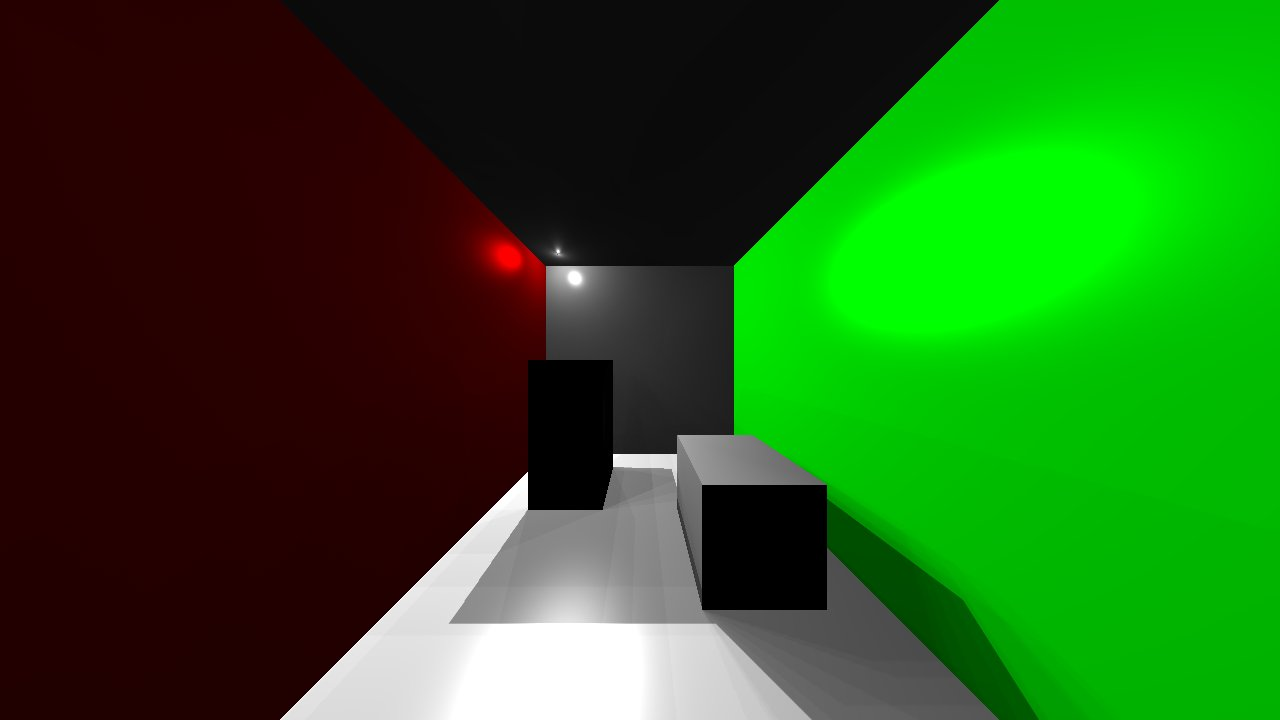
\includegraphics[width=\textwidth]{sample2.jpg}
%                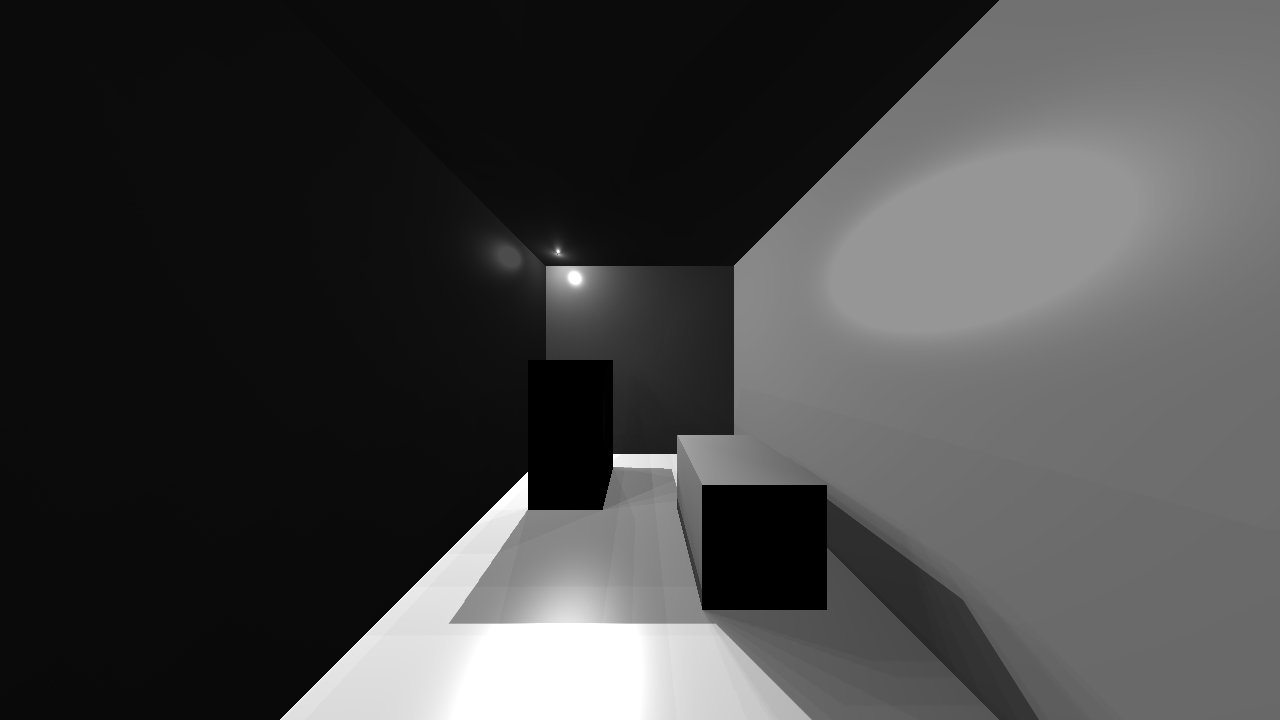
\includegraphics[width=\textwidth]{sample2_gray.jpg}
                \caption{Light is at the far upper left corner of the scene.}
                \label{fig:sample2}
        \end{subfigure}
        \begin{subfigure}[b]{0.5\textwidth}
                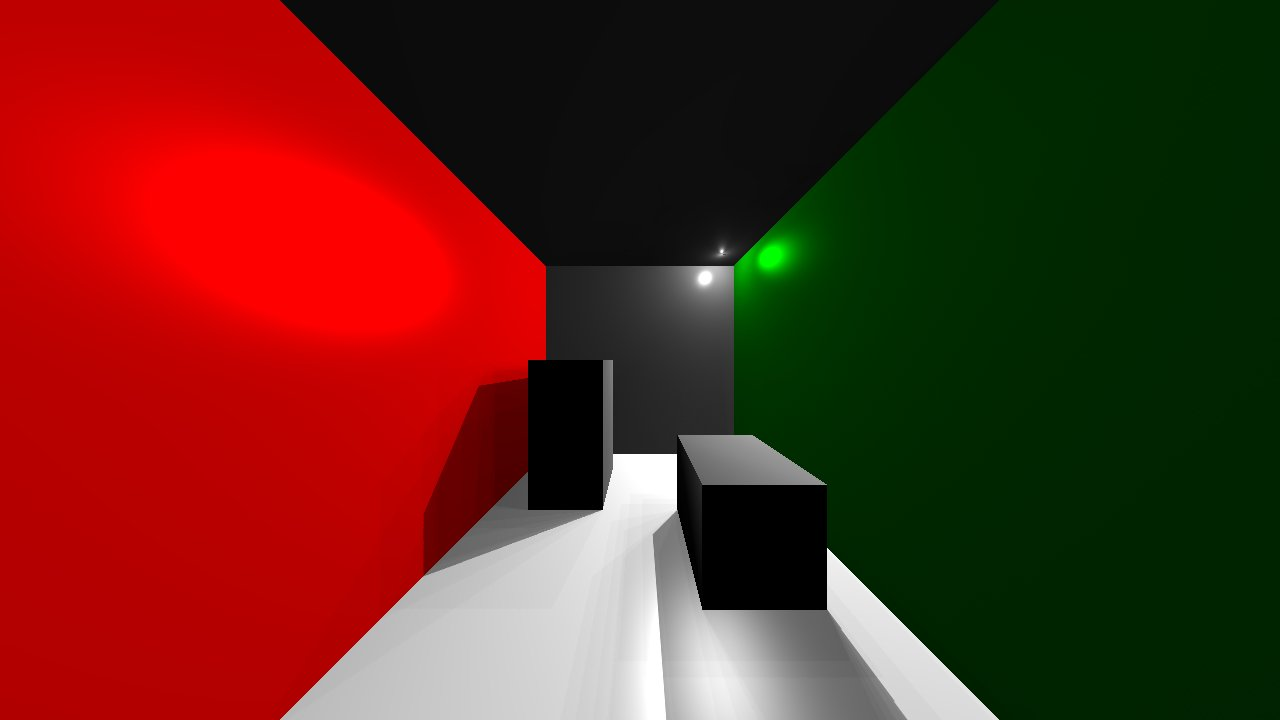
\includegraphics[width=\textwidth]{sample3.jpg}
%                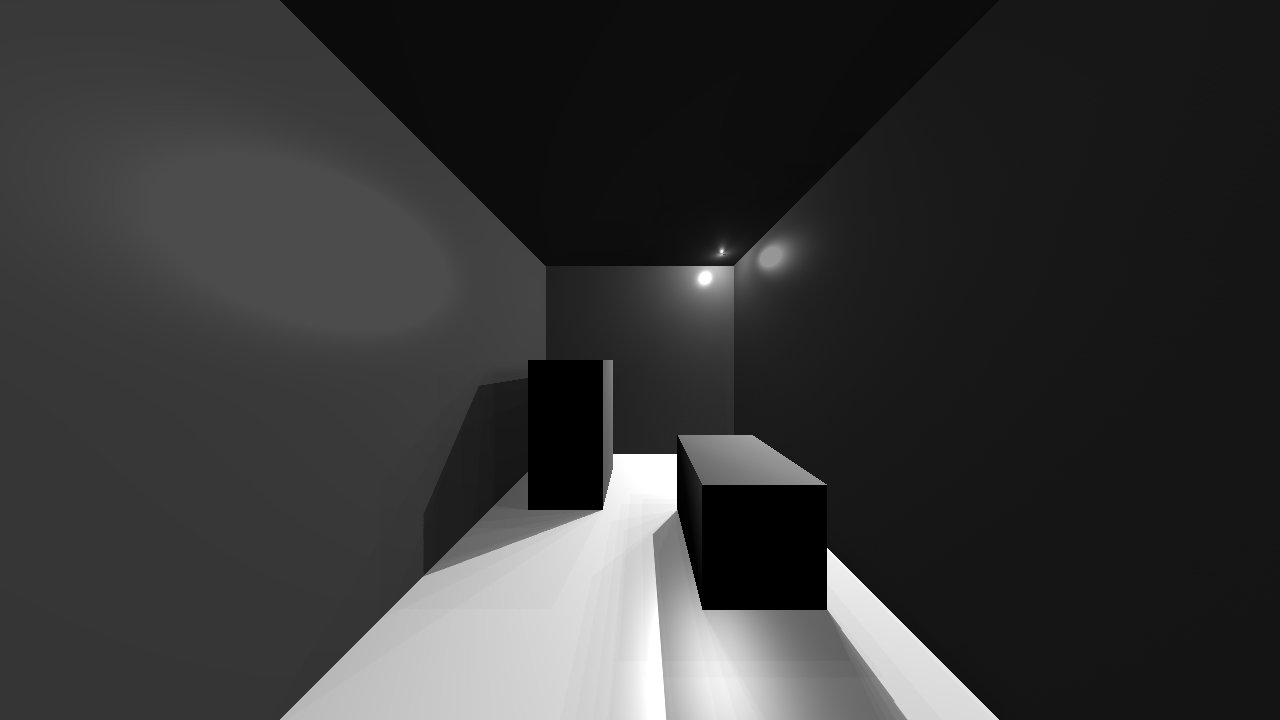
\includegraphics[width=\textwidth]{sample3_gray.jpg}
                \caption{Light is at the far upper right corner of the scene.}
                \label{fig:sample3}
        \end{subfigure}
        \begin{subfigure}[b]{0.5\textwidth}
                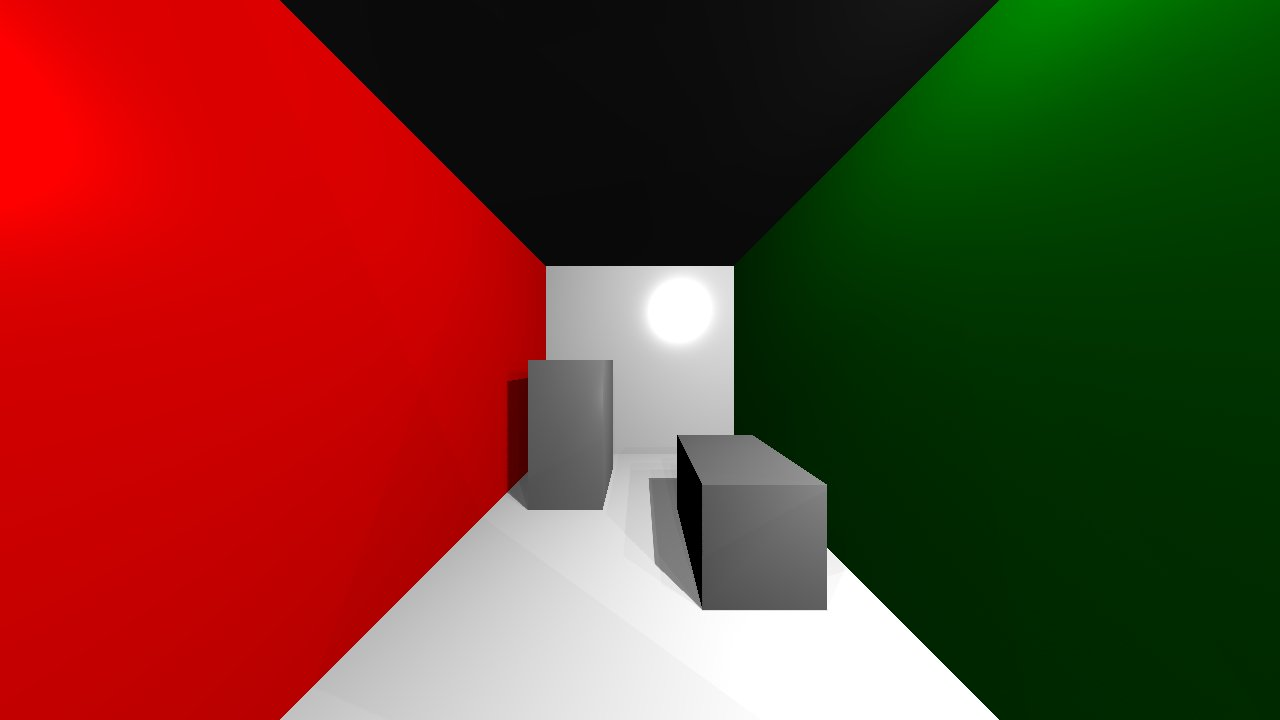
\includegraphics[width=\textwidth]{sample4.jpg}
%                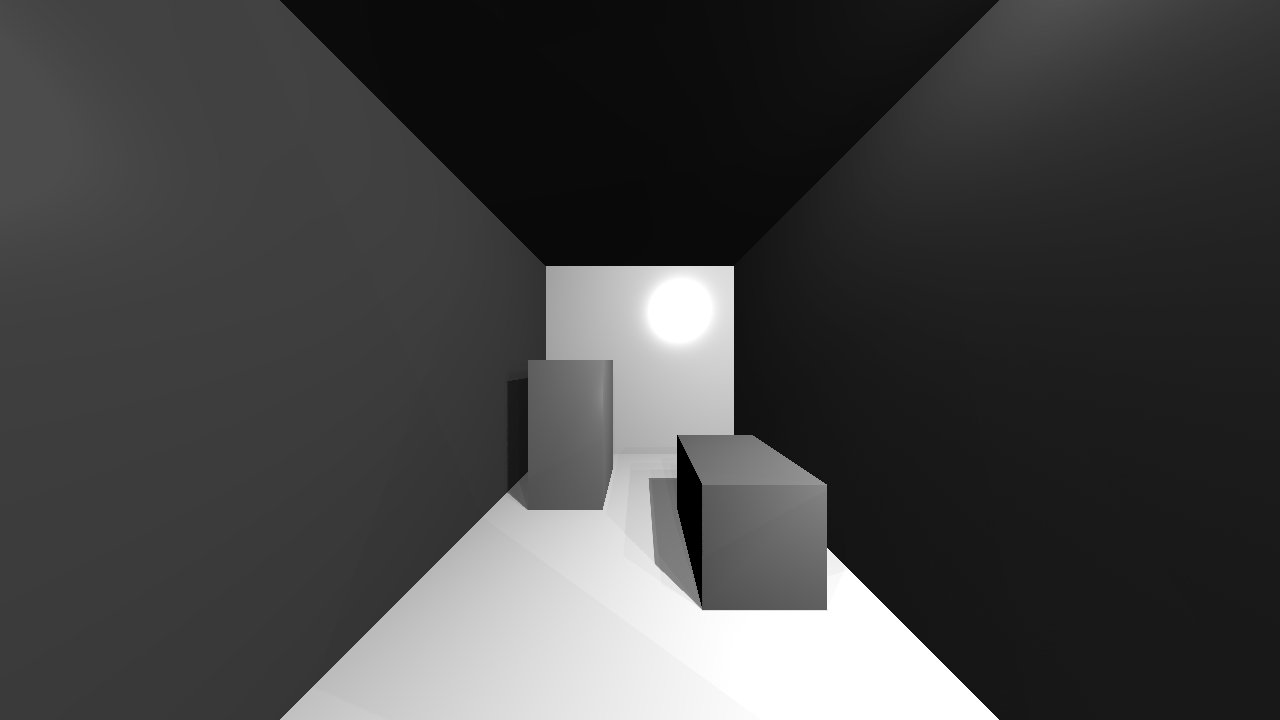
\includegraphics[width=\textwidth]{sample4_gray.jpg}
                \caption{Light is at the near upper right corner of the scene.}
                \label{fig:sample4}
        \end{subfigure}
        \begin{subfigure}[b]{0.5\textwidth}
                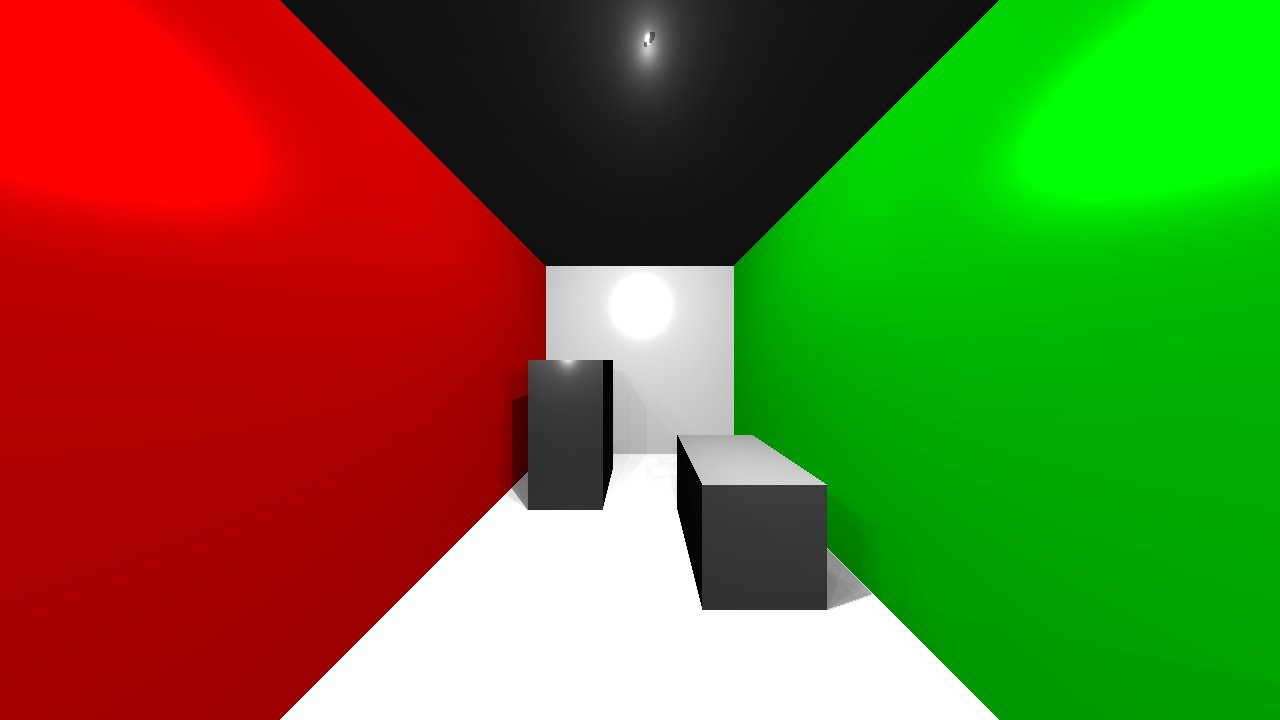
\includegraphics[width=\textwidth]{sample5.jpg}
%                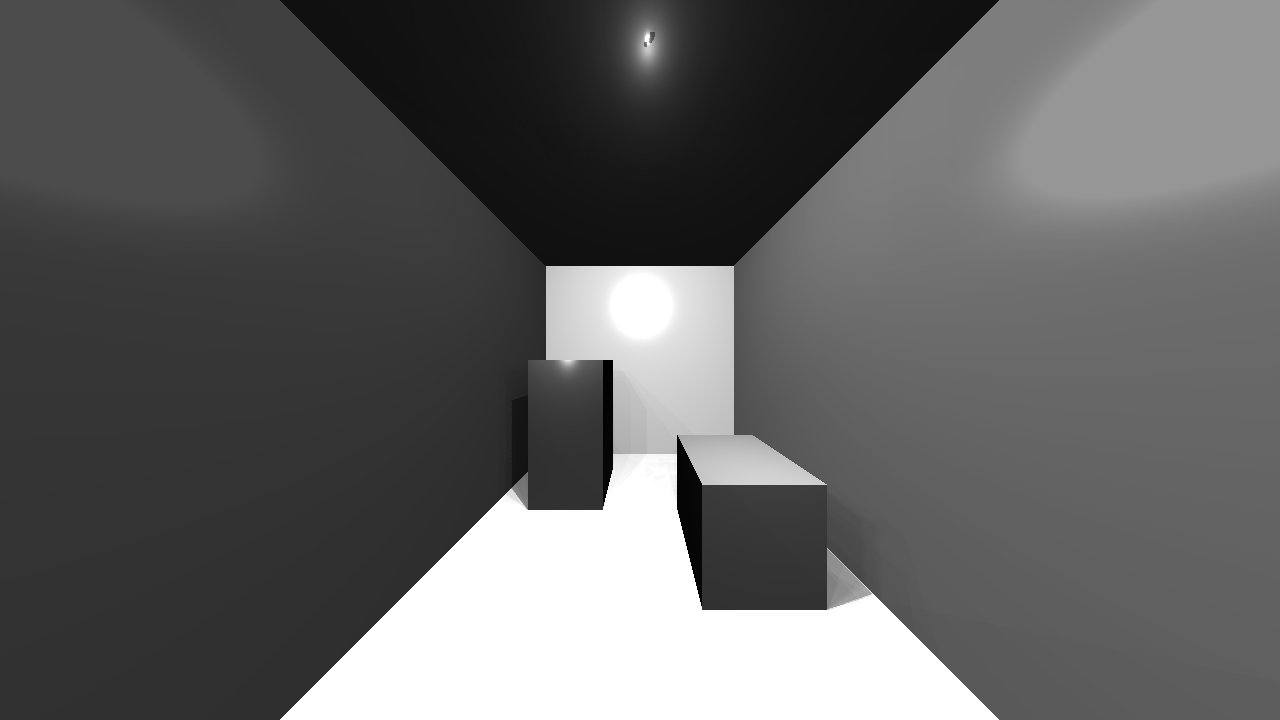
\includegraphics[width=\textwidth]{sample5_gray.jpg}
                \caption{Light is in the upper center of the scene.}
                \label{fig:sample5}
        \end{subfigure}
        \caption{Additional Rendered Images Using the Default Parameters}\label{fig:default}
\end{figure}


\begin{figure}[h!]
  \centering
    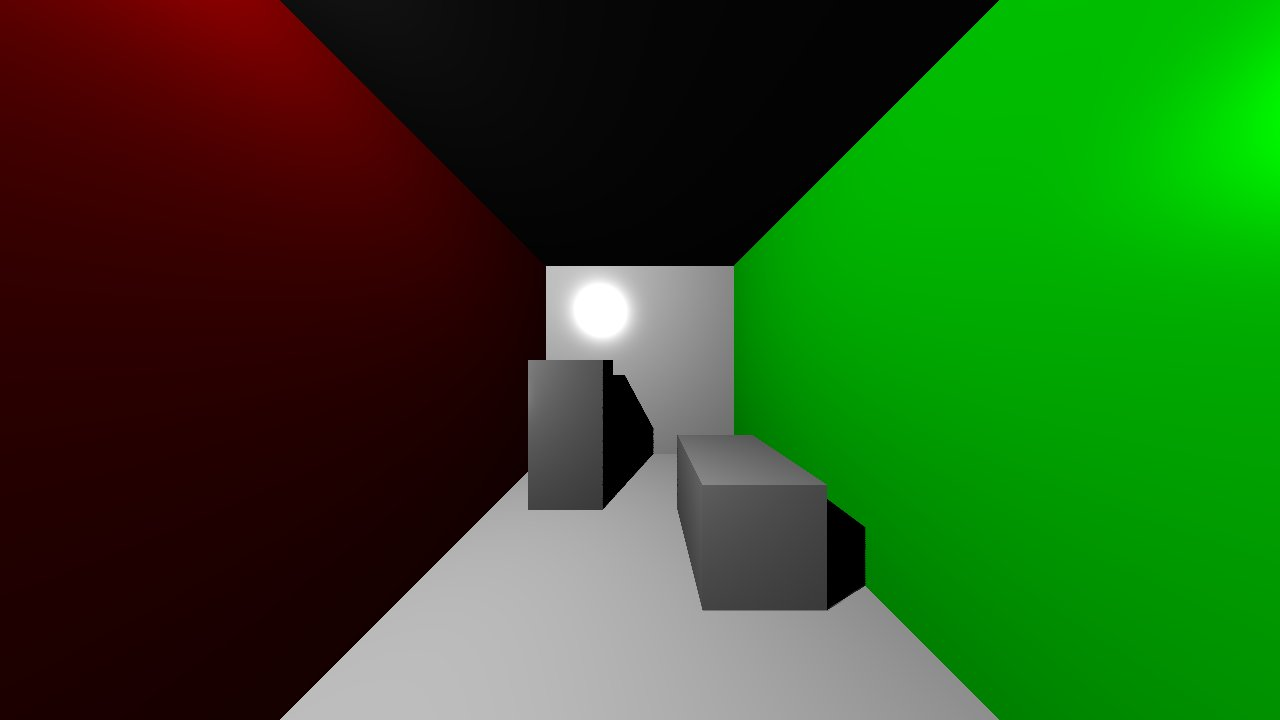
\includegraphics[width=1.0\textwidth]{direct_only.jpg}
%    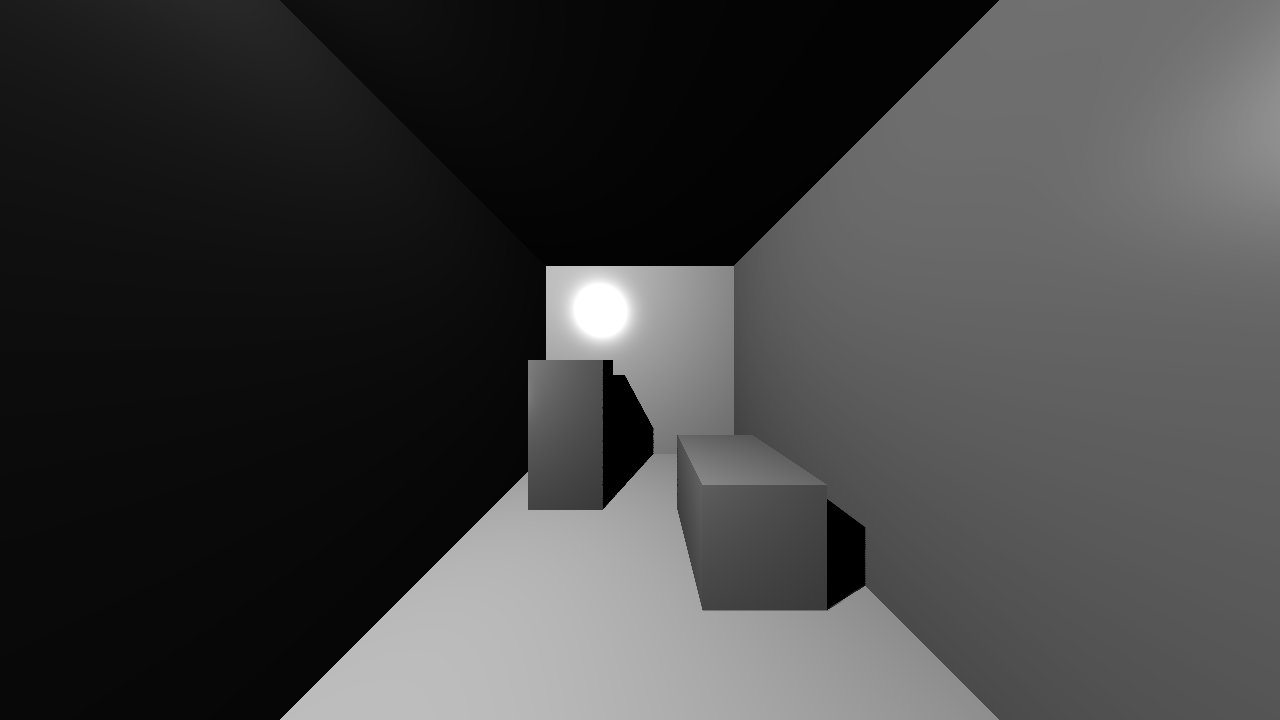
\includegraphics[width=1.0\textwidth]{direct_only_gray.jpg}
    \caption{Scene rendered with only direct lighting.}
	\label{fig:directonly}
\end{figure}


\begin{figure}
        \centering
        \begin{subfigure}[b]{1.0\textwidth}
                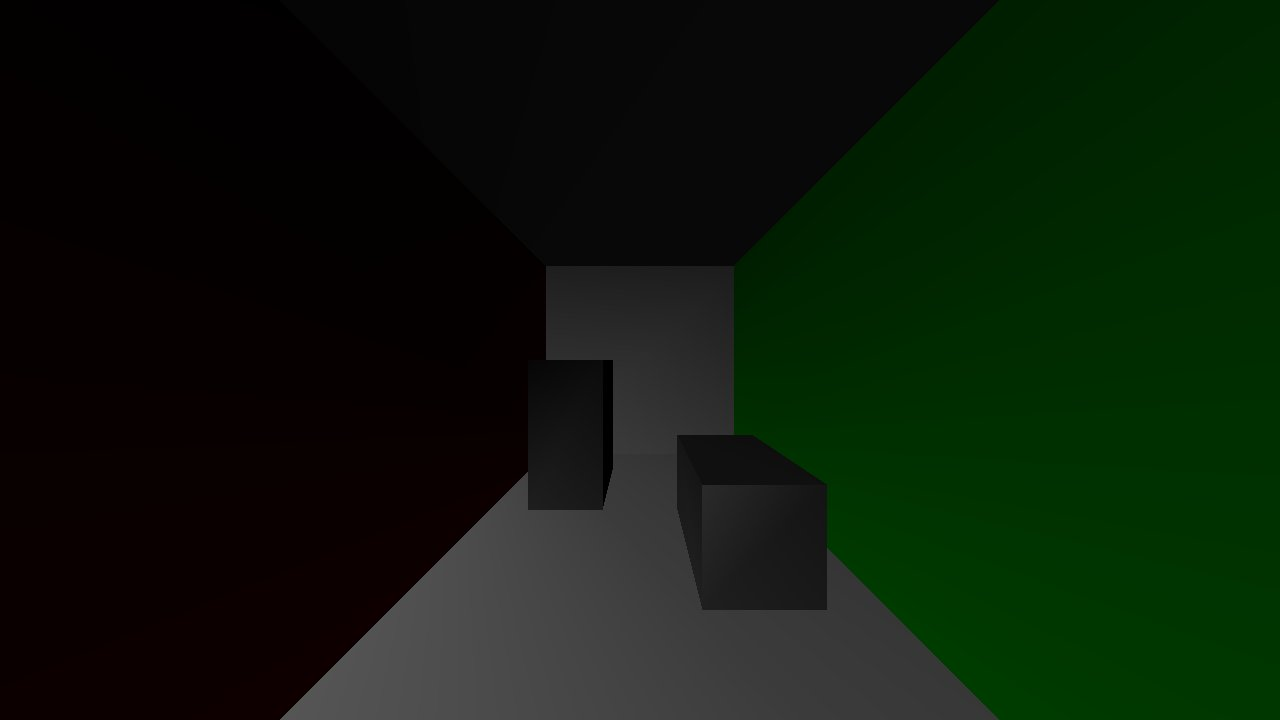
\includegraphics[width=\textwidth]{indirect_only.jpg}
%                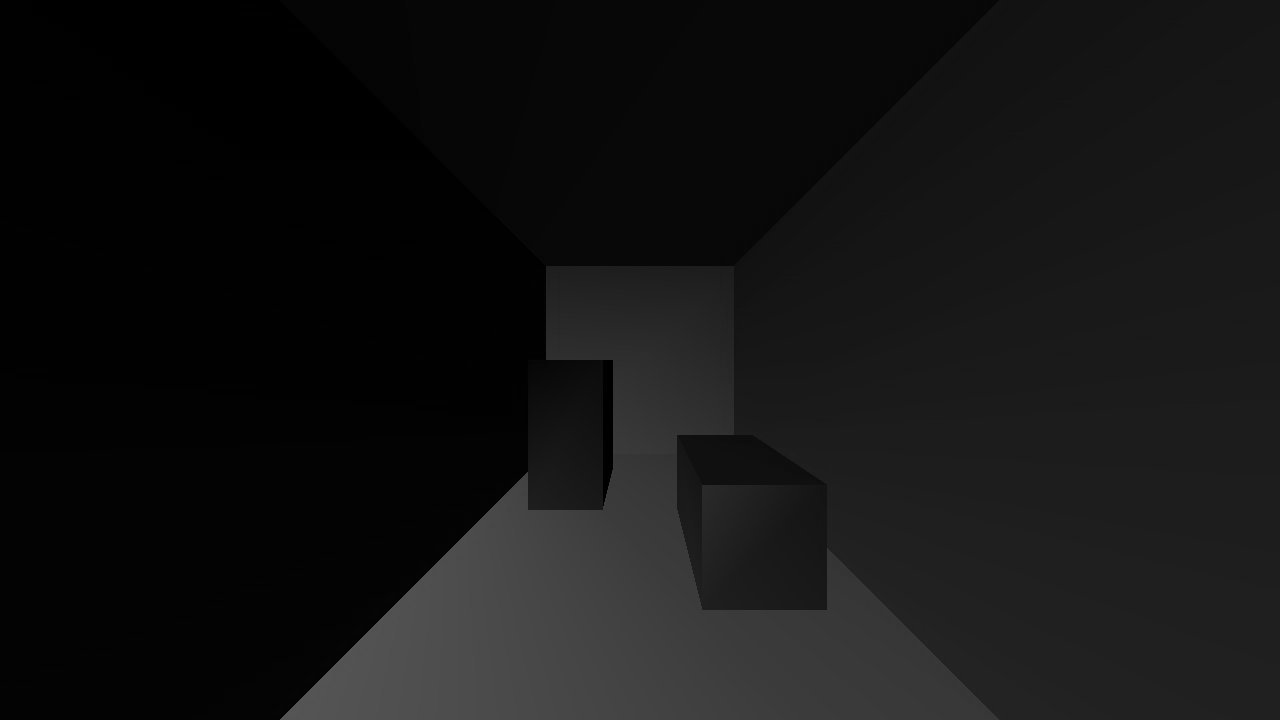
\includegraphics[width=\textwidth]{indirect_only_gray.jpg}
                \caption{Indirect Lighting Only w/out Indirect Shadows}
                \label{fig:indirectonly}
        \end{subfigure}
        \begin{subfigure}[b]{1.0\textwidth}
                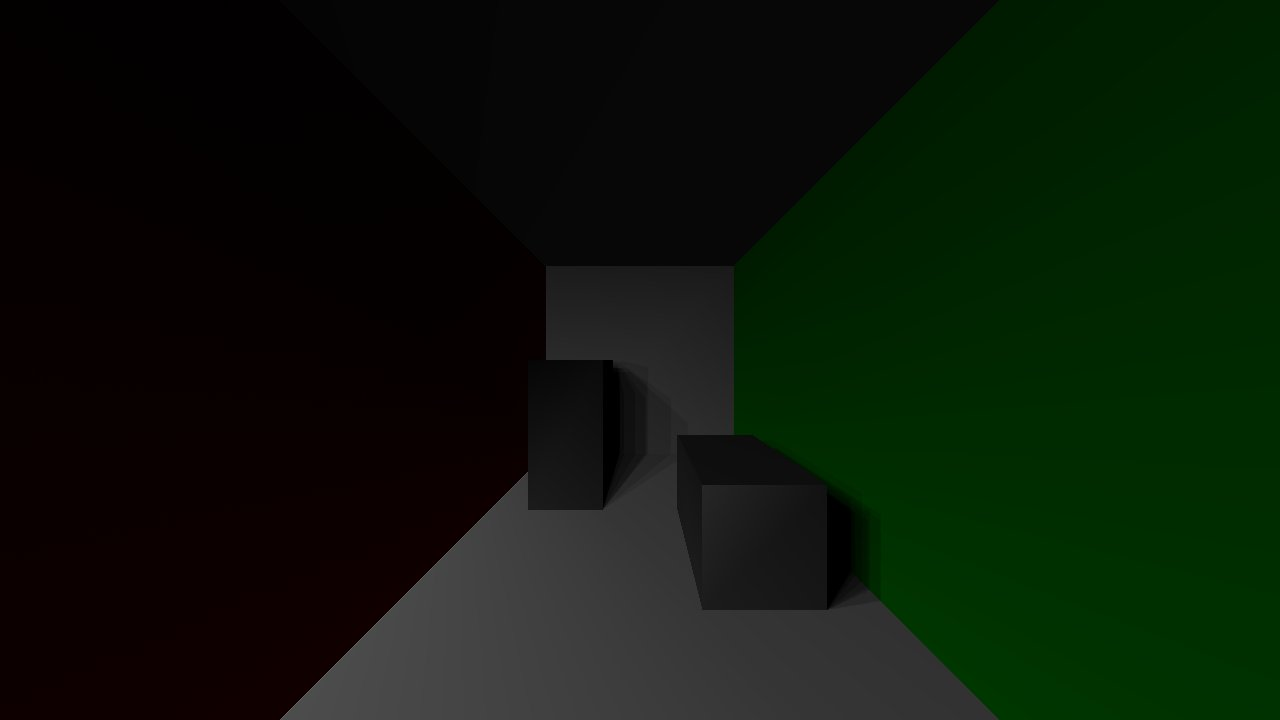
\includegraphics[width=\textwidth]{indirect_only_shadows.jpg}
%                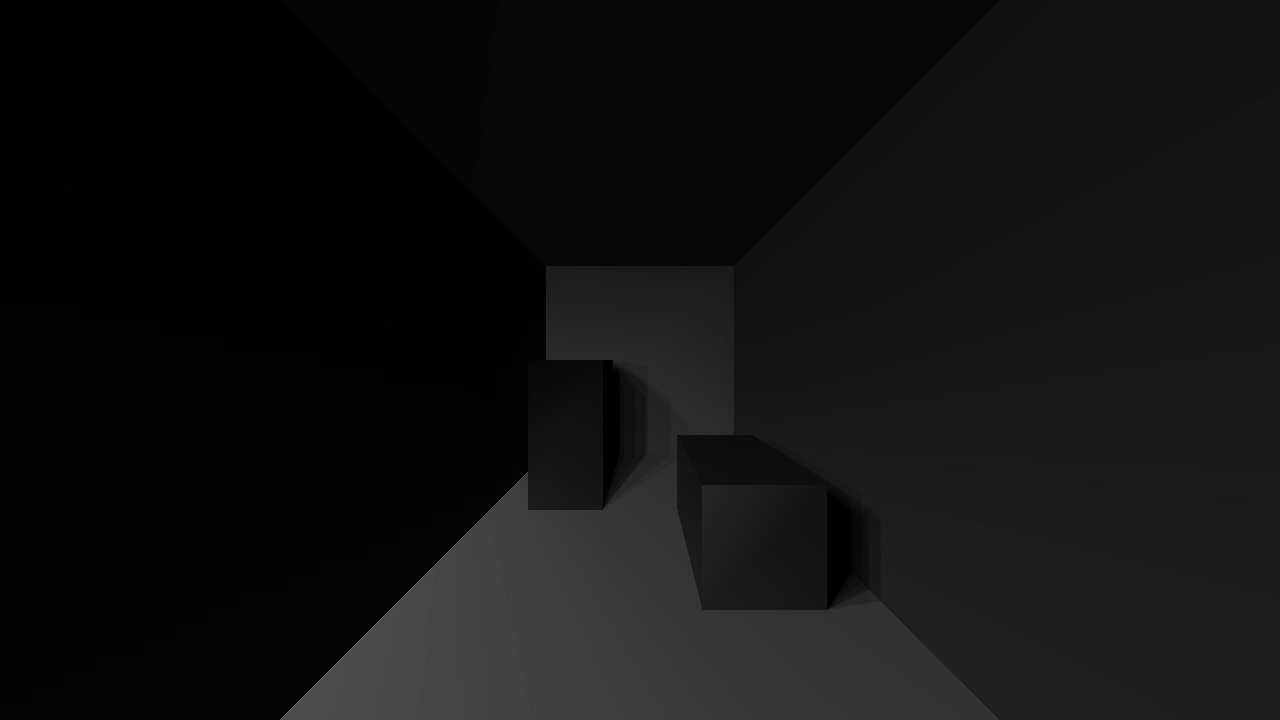
\includegraphics[width=\textwidth]{indirect_only_shadows_gray.jpg}
                \caption{Indirect Lighting Only w/ Indirect Shadows}
                \label{fig:indirectonlyshadows}
        \end{subfigure}
        \caption{Images showing the contributions from the VPL's to indirect lighting.}\label{fig:indirect}
\end{figure}


\begin{figure}
        \centering
        \begin{subfigure}[b]{0.75\textwidth}
                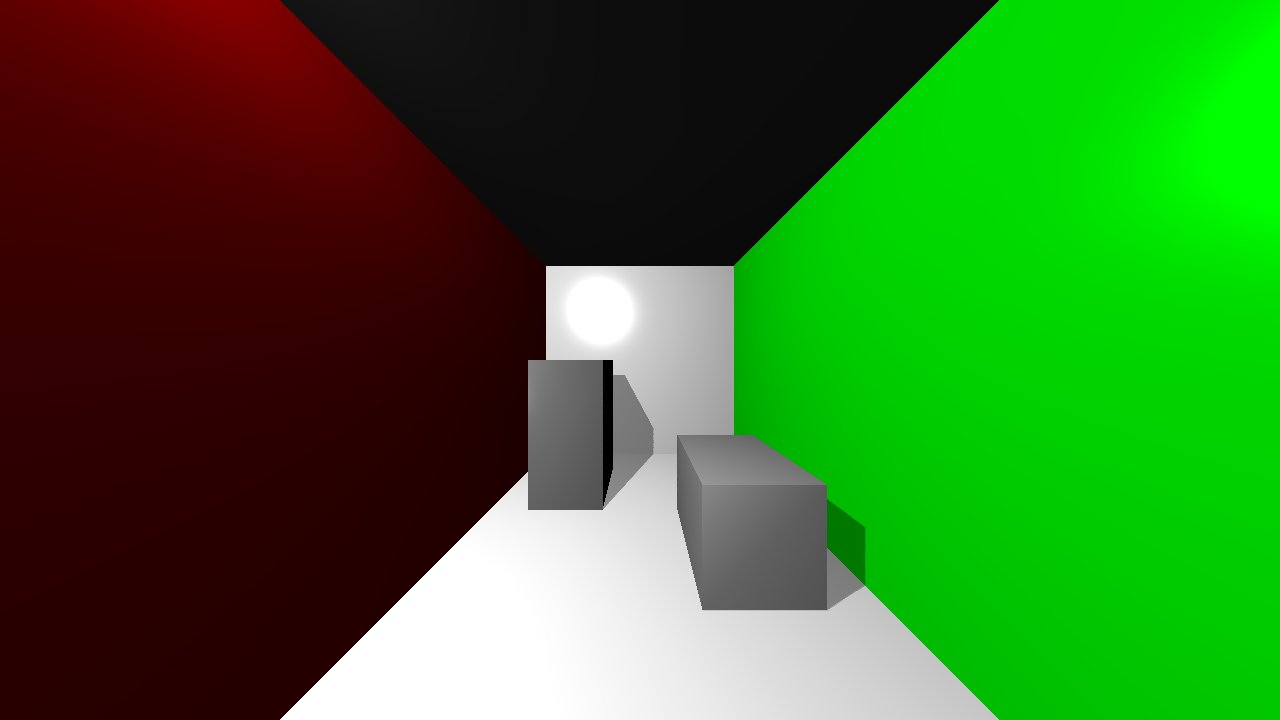
\includegraphics[width=\textwidth]{23.jpg}
%                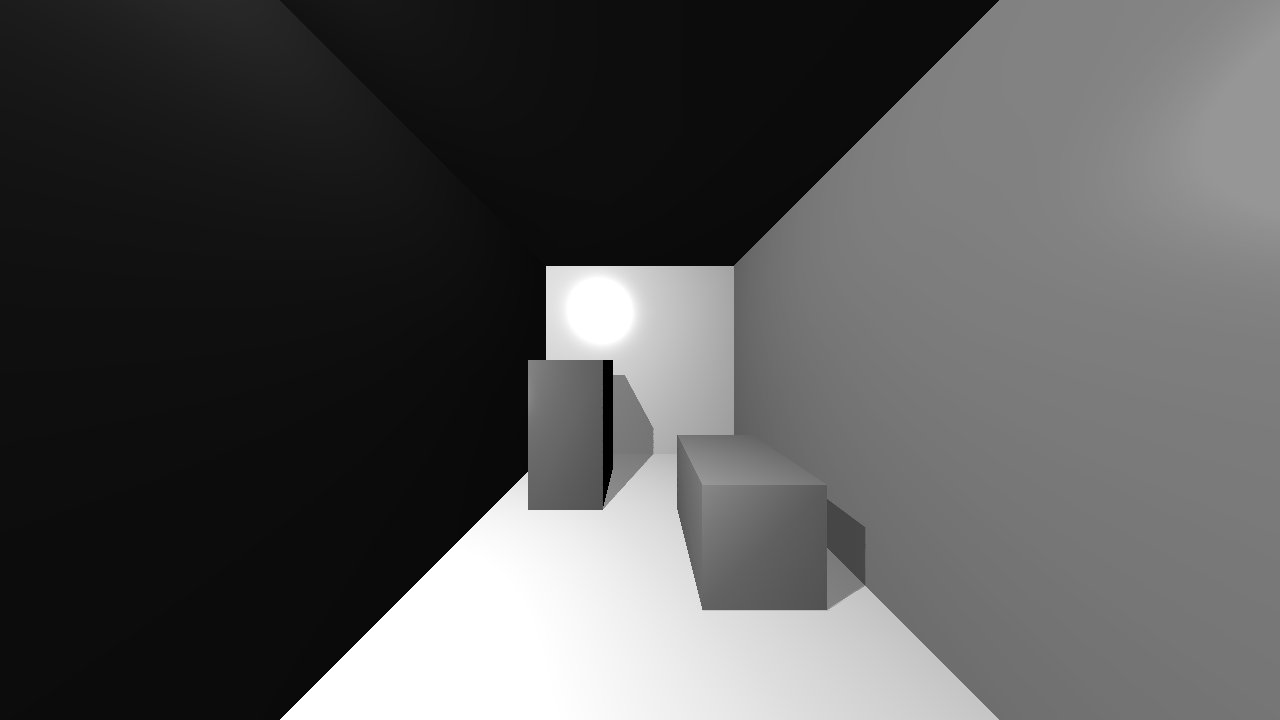
\includegraphics[width=\textwidth]{23_gray.jpg}
                \caption{Scene Rendered with Indirect Lighting w/out Indirect Shadows.}
                \label{fig:0indSM}
        \end{subfigure}
        \begin{subfigure}[b]{0.75\textwidth}
                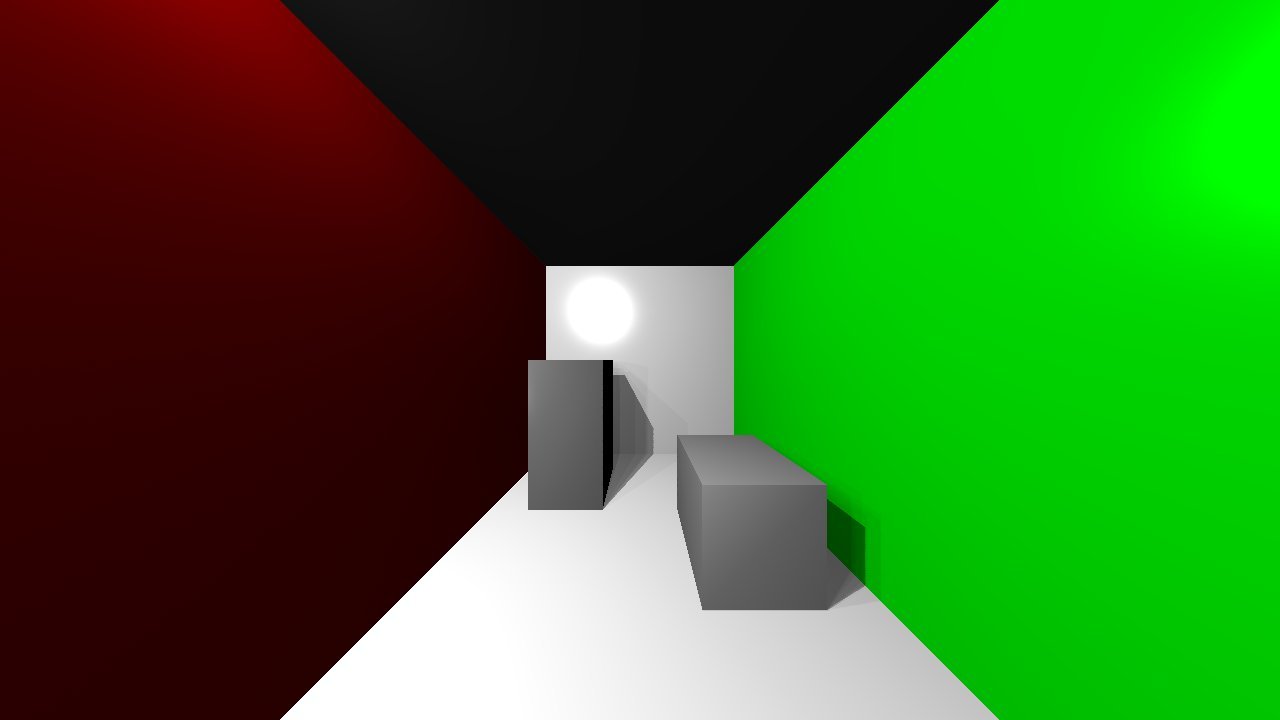
\includegraphics[width=\textwidth]{19.jpg}
%                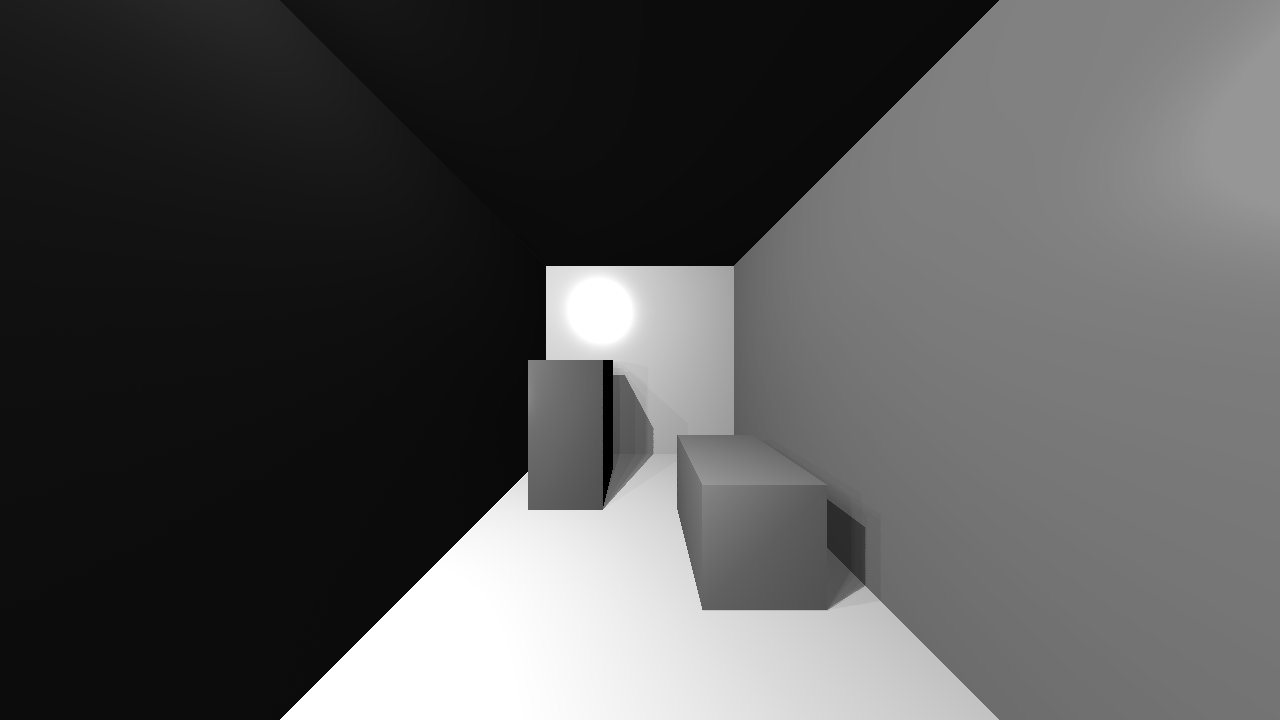
\includegraphics[width=\textwidth]{19_gray.jpg}
                \caption{Scene Rendered with Indirect Lighting w/ 15 Indirect Shadow Maps.}
                \label{fig:15indSM}
        \end{subfigure}
        \begin{subfigure}[b]{0.75\textwidth}
                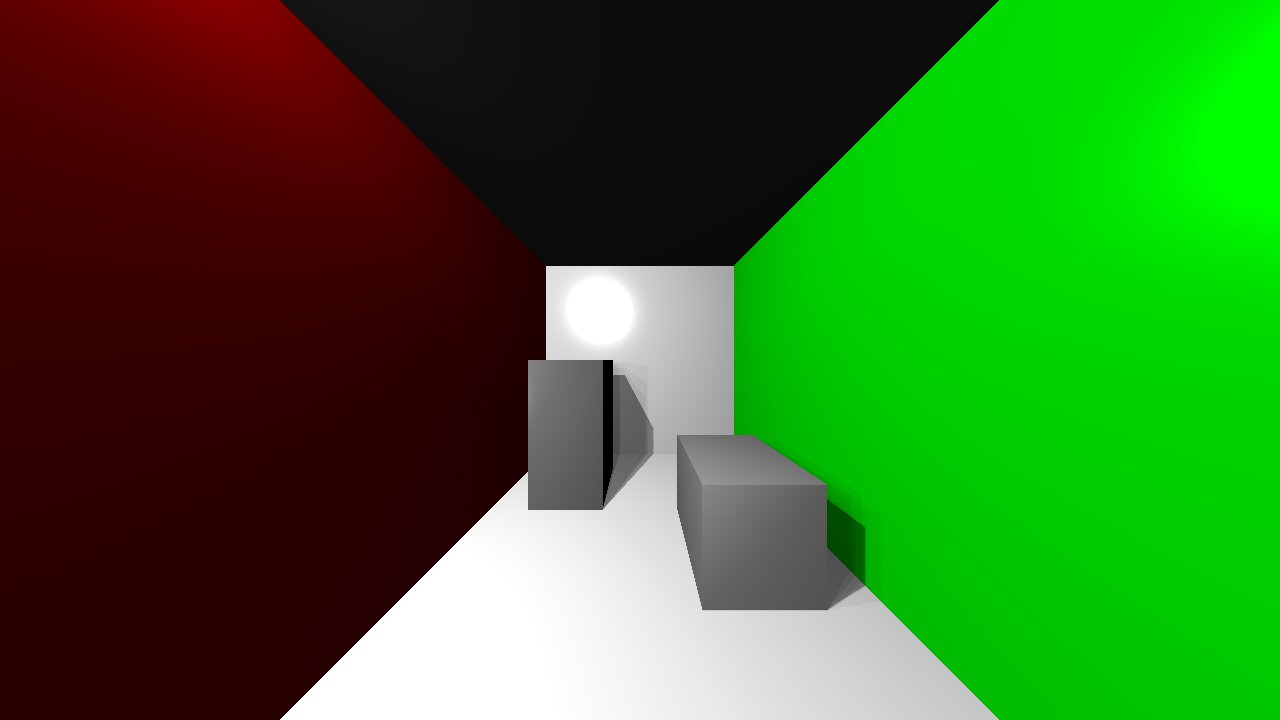
\includegraphics[width=\textwidth]{20.jpg}
%                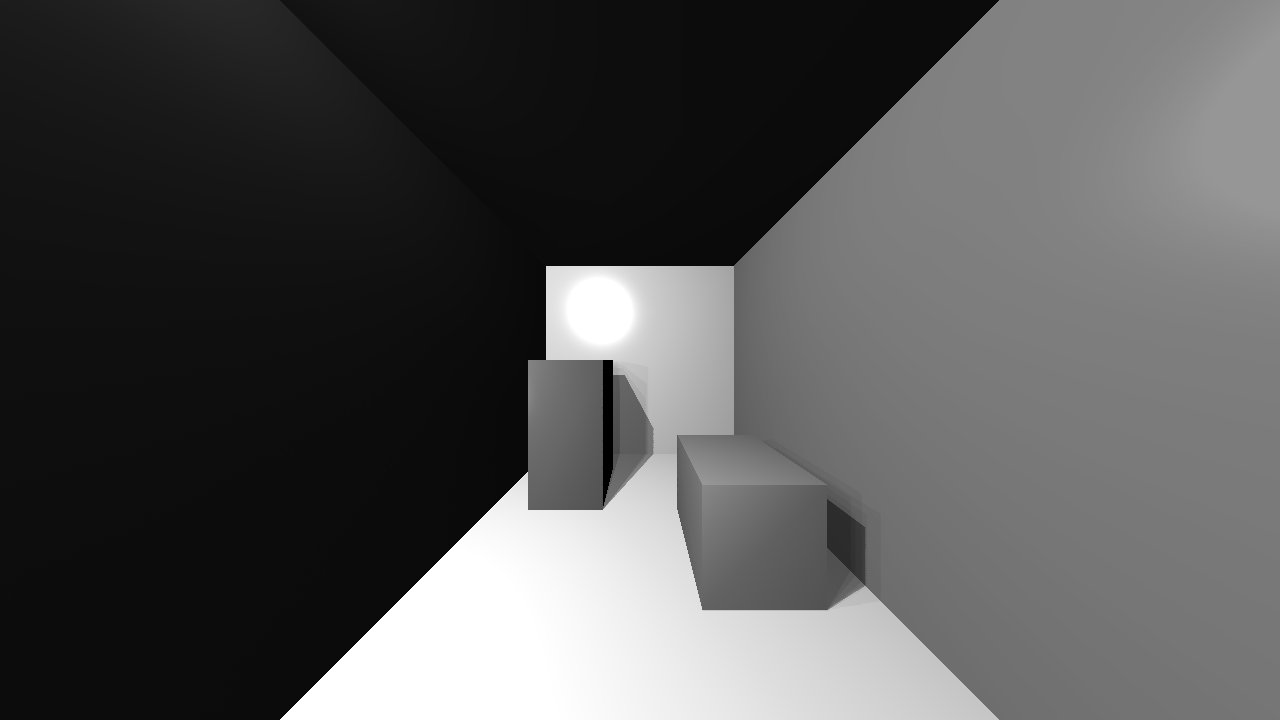
\includegraphics[width=\textwidth]{20_gray.jpg}
                \caption{Scene Rendered with Indirect Lighting w/ 10 Indirect Shadow Maps.}
                \label{fig:10indSM}
        \end{subfigure}
        \caption{Varying Indirect Lighting Adjustments} \label{fig:indirectimages}
\end{figure}


\begin{figure}[h!]
  \centering
    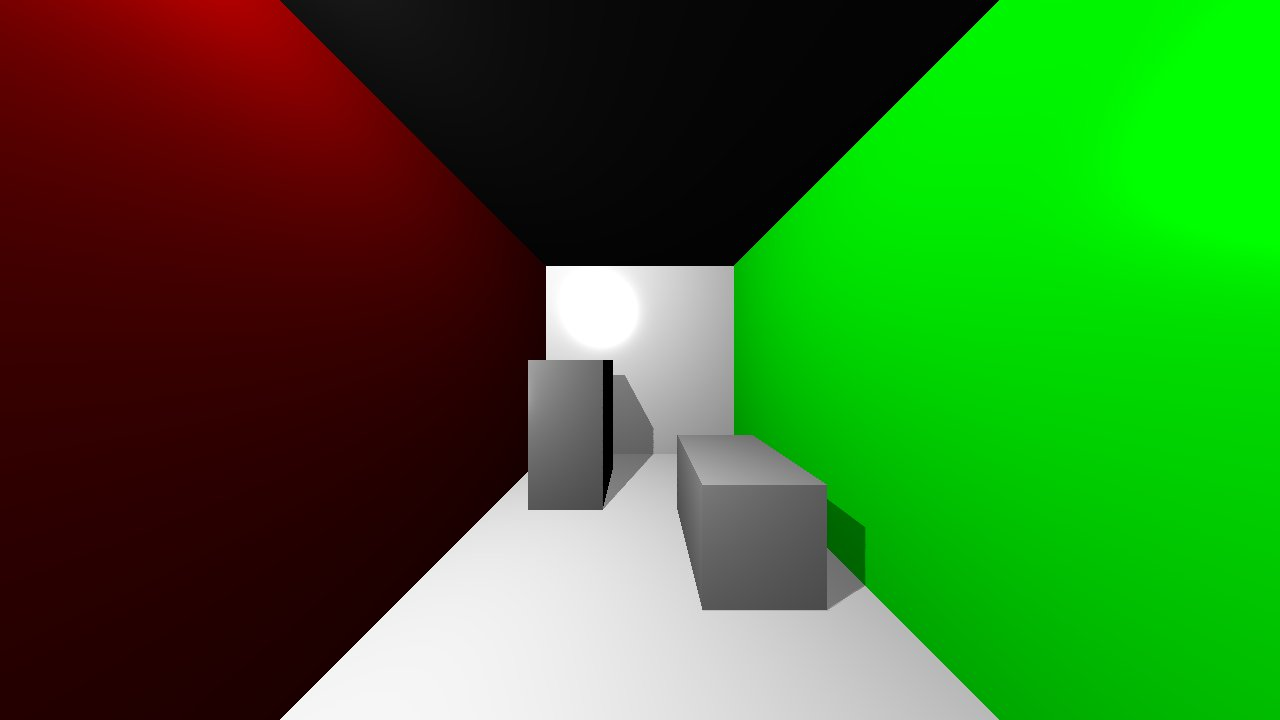
\includegraphics[width=1.0\textwidth]{direct_only_fake_1_3.jpg}
%    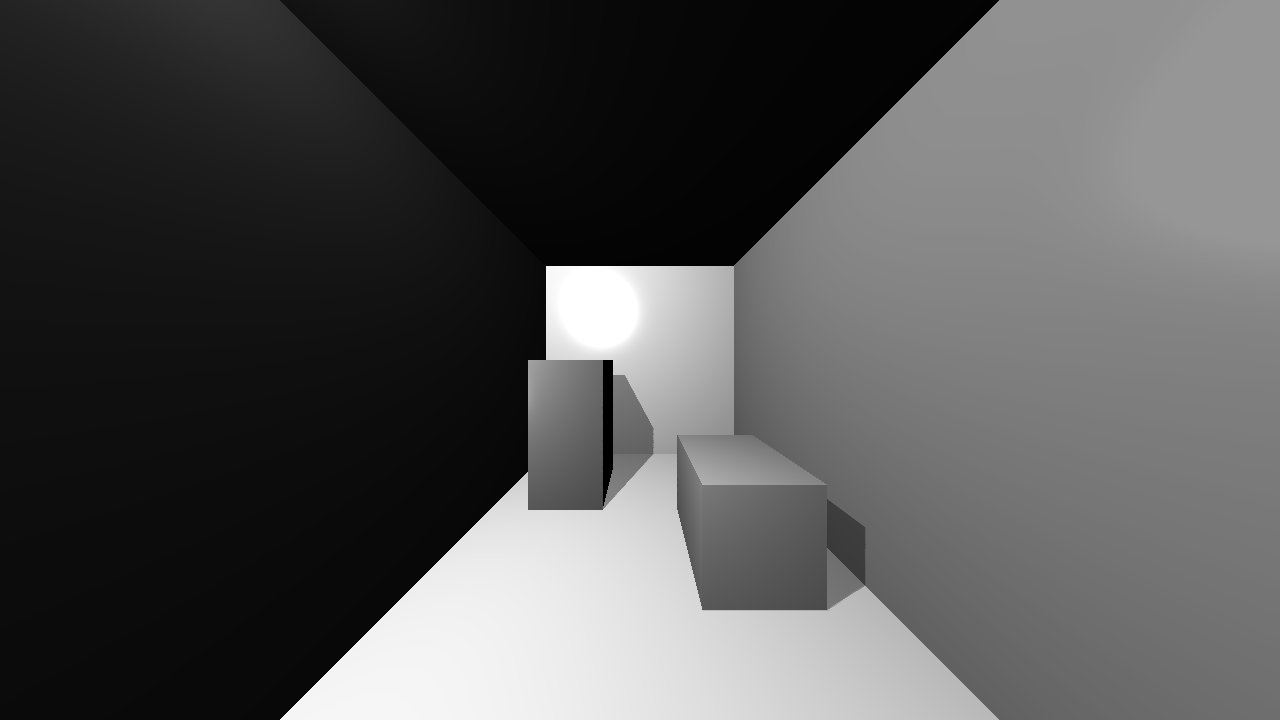
\includegraphics[width=1.0\textwidth]{direct_only_fake_1_3_gray.jpg}
  \caption{Faked Indirect Lighting with a 1.3x Multiplier.}
	\label{fig:fakedindirect}
\end{figure}


\begin{figure}
        \centering
        \begin{subfigure}[b]{1.0\textwidth}
                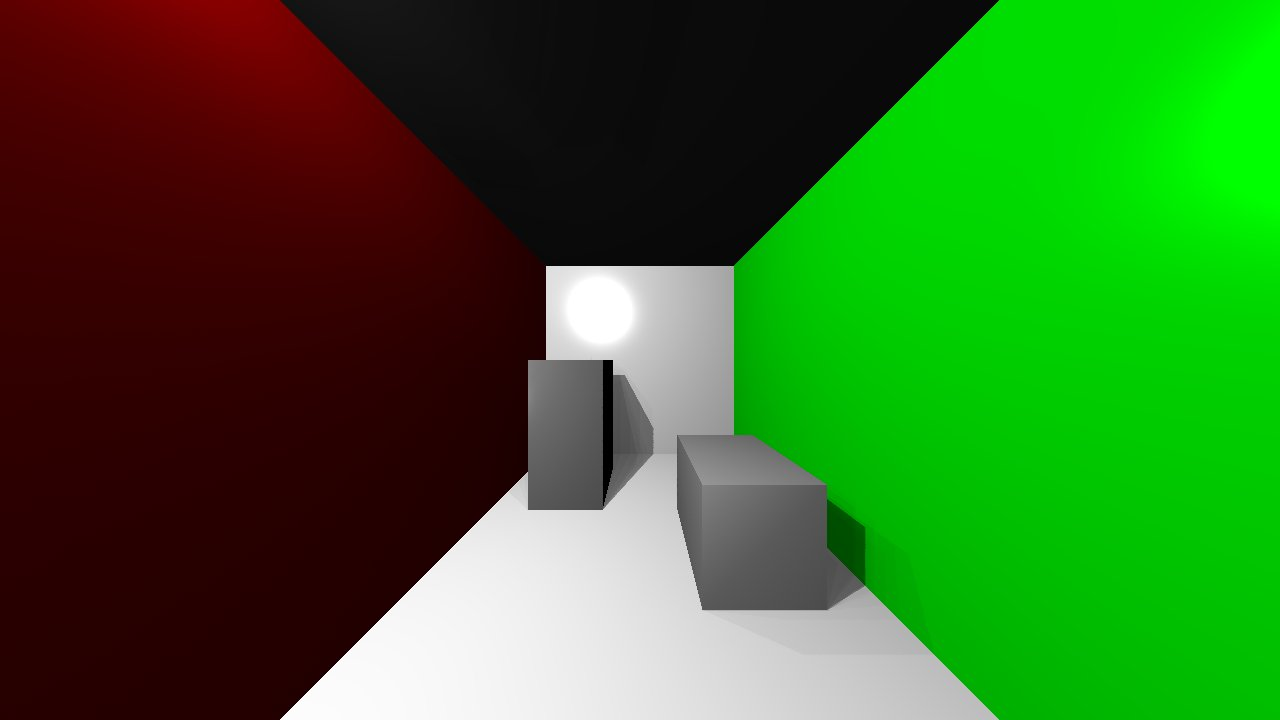
\includegraphics[width=\textwidth]{3.jpg}
%                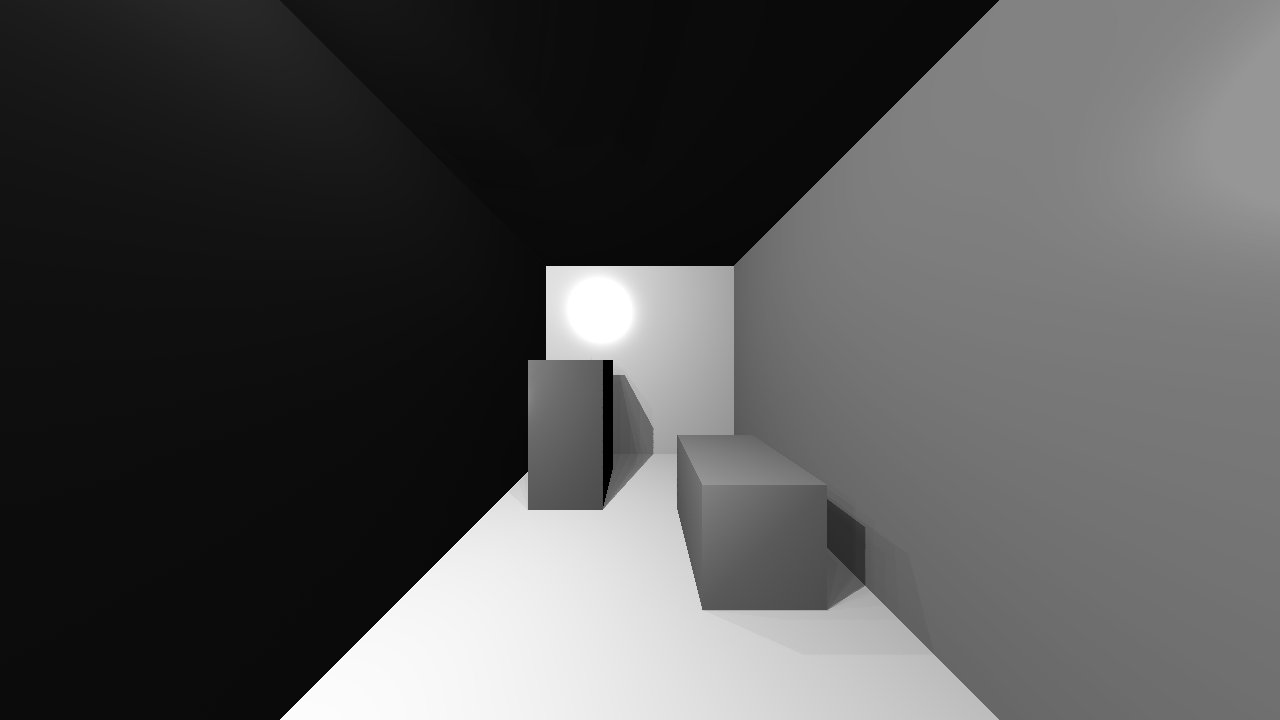
\includegraphics[width=\textwidth]{3_gray.jpg}
                \caption{30 Degree Angle Between VPL Rays.}
                \label{fig:VPLangleIncrease}
        \end{subfigure}
        \begin{subfigure}[b]{1.0\textwidth}
                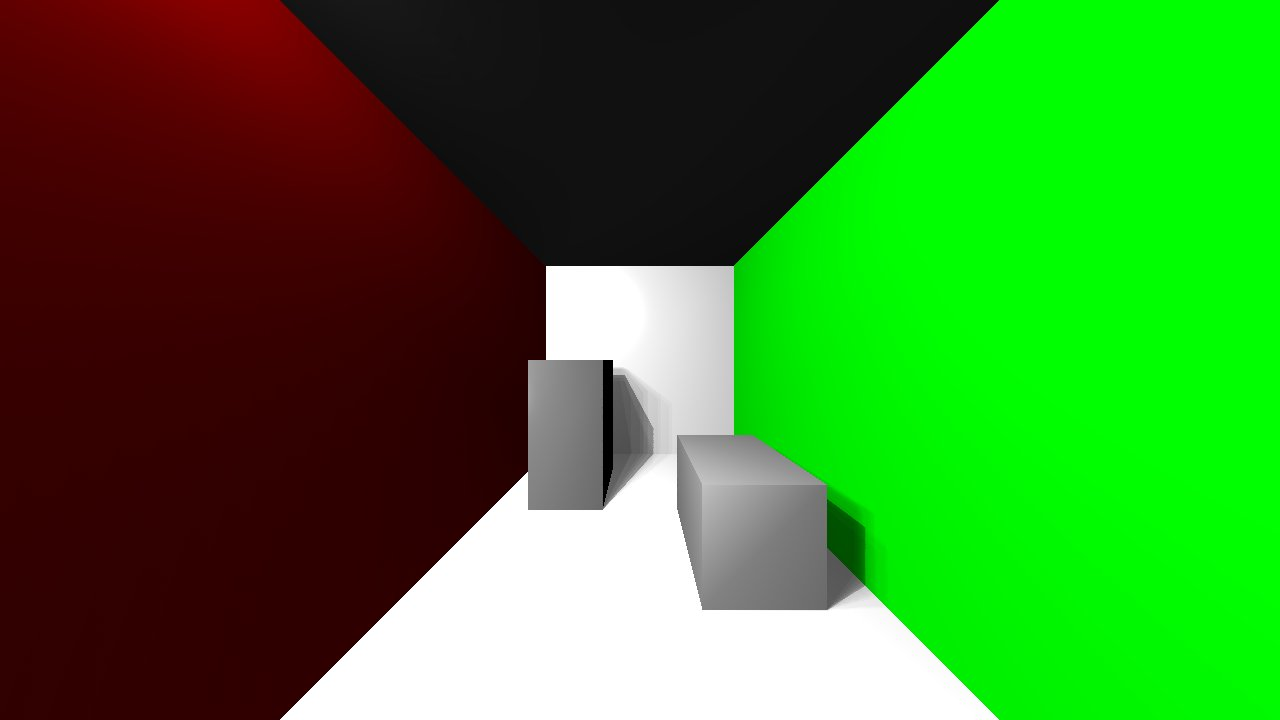
\includegraphics[width=\textwidth]{7.jpg}
%                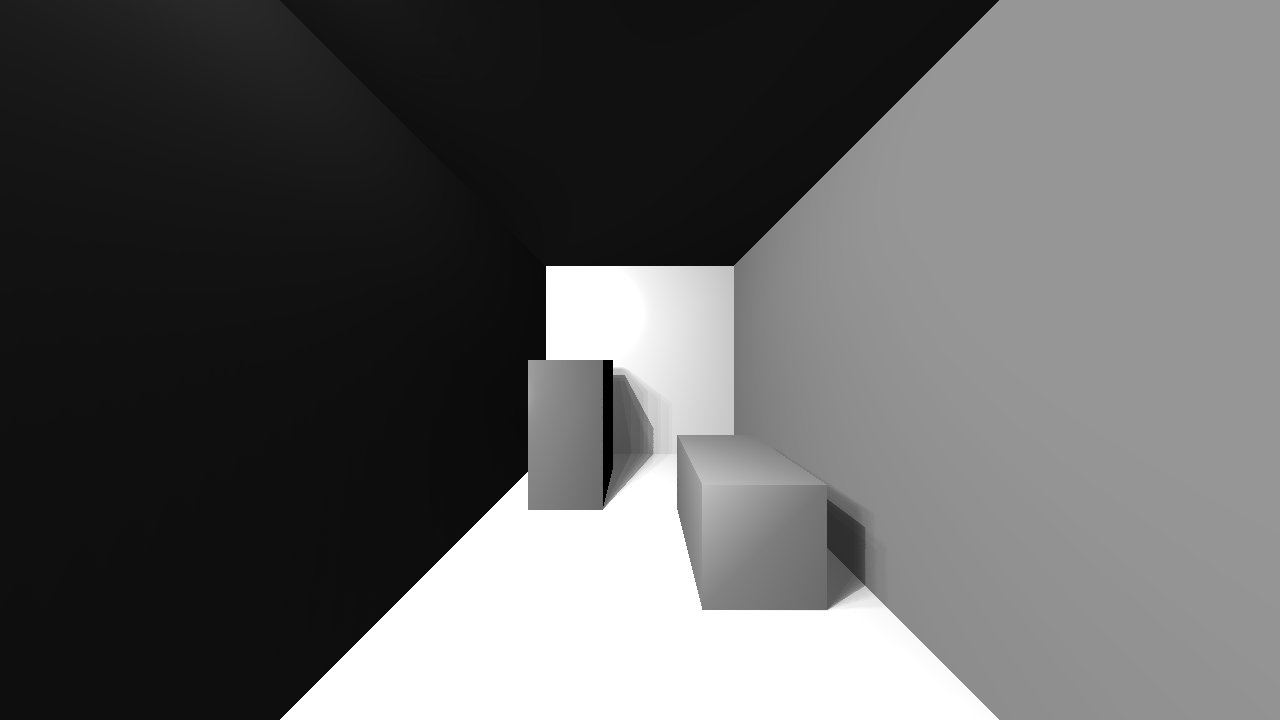
\includegraphics[width=\textwidth]{7_gray.jpg}
                \caption{Reduction down to 1 VPL Per Ray (1 Hemisphere)}
                \label{fig:hemisphereReduction}
        \end{subfigure}
        \caption{Adjusting VPL parameters}\label{fig:vplparameters}
\end{figure}


\begin{figure}
        \centering
        \begin{subfigure}[b]{1.0\textwidth}
                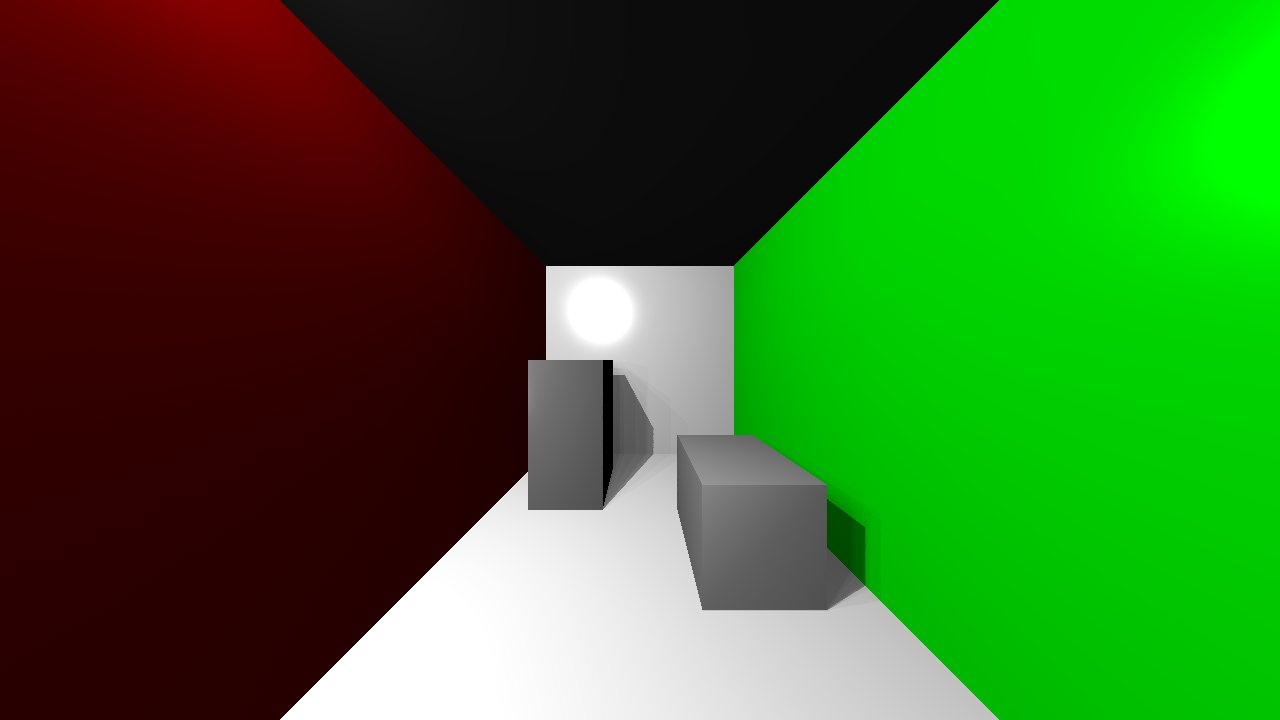
\includegraphics[width=\textwidth]{sample1.jpg}
%                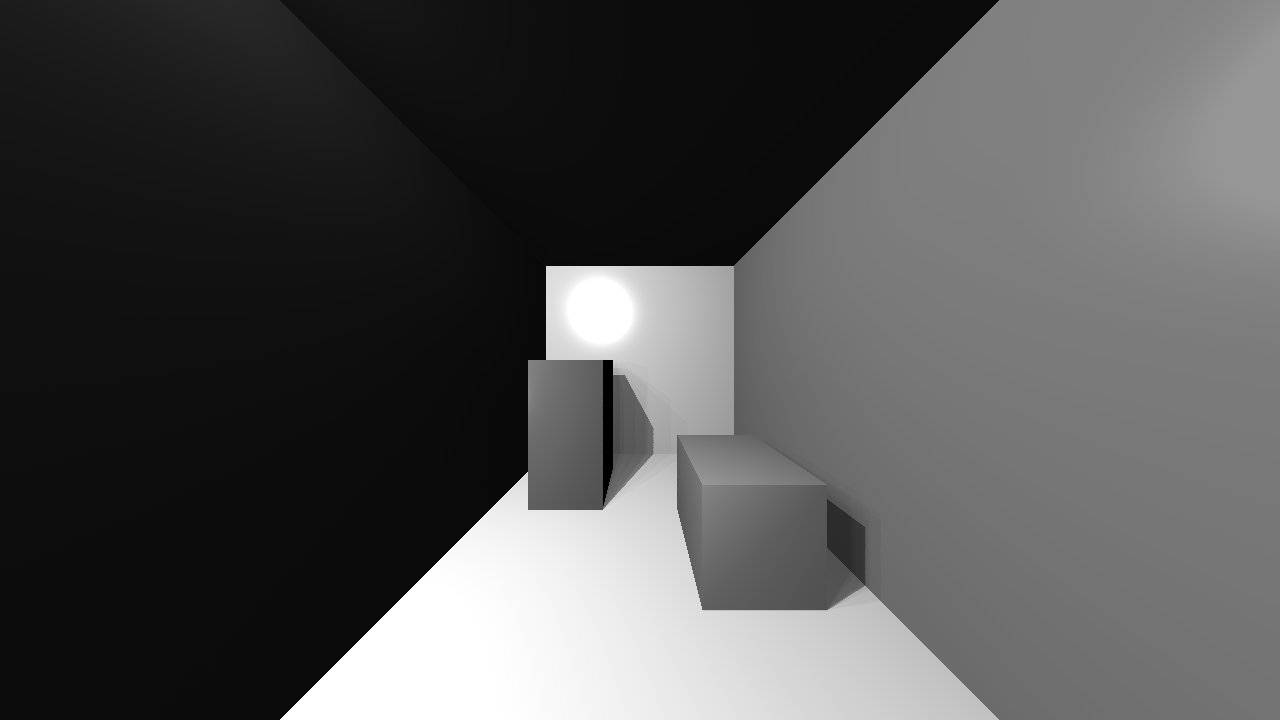
\includegraphics[width=\textwidth]{sample1_gray.jpg}
                \caption{Default Resolution.}
                \label{fig:defaultresolution}
        \end{subfigure}
        \begin{subfigure}[b]{1.0\textwidth}
                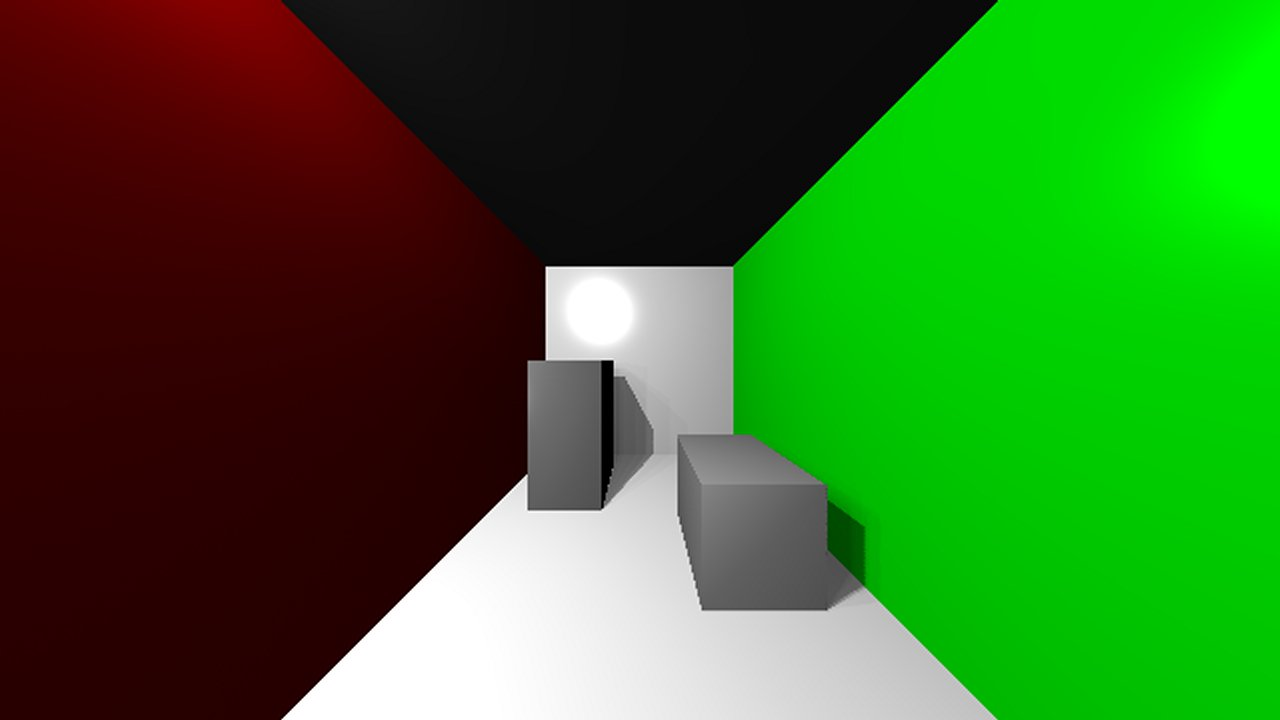
\includegraphics[width=\textwidth]{17_resize.jpg}
%                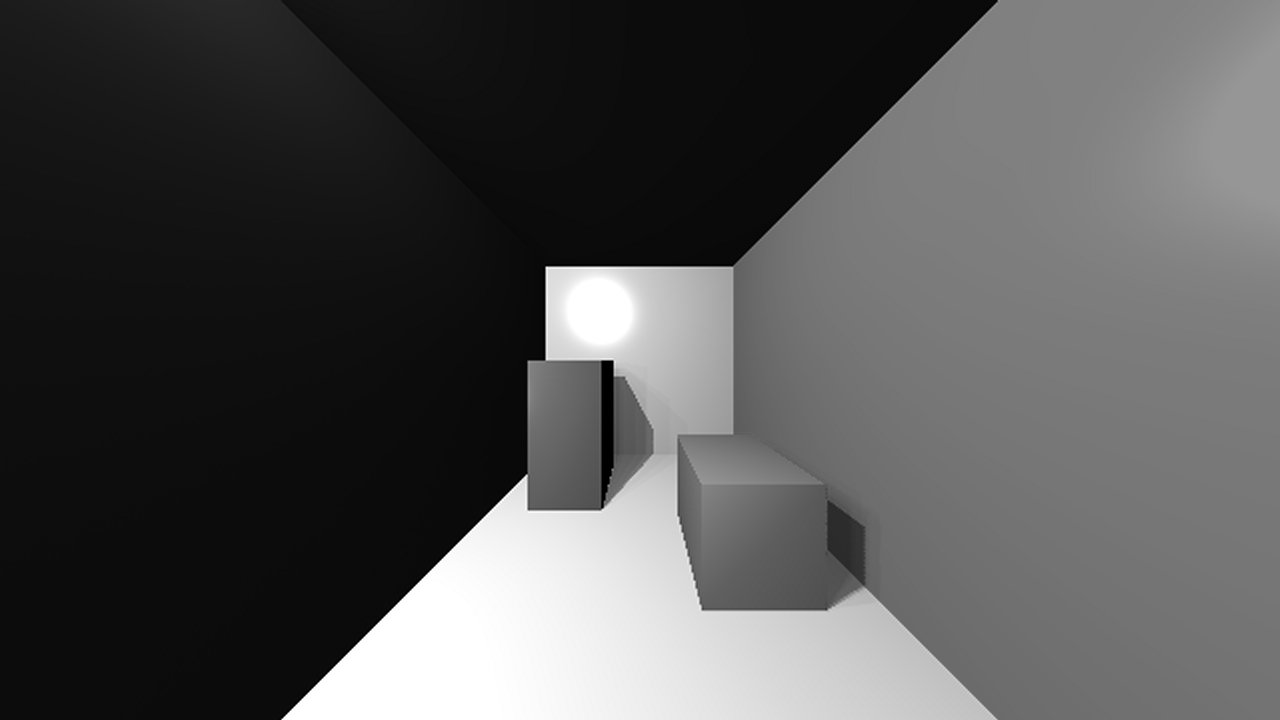
\includegraphics[width=\textwidth]{17_resize_gray.jpg}
                \caption{Smaller Resolution Stretched to Default Size}
                \label{fig:smallerresolution}
        \end{subfigure}
        \caption{Comparison of default resolution and a smaller resolution stretched.}\label{fig:artifacts}
\end{figure}



